\section{Introduction}\label{sec:WBoson_Introduction}

This section provides a short introduction to the \Wb-boson analysis. It starts with a brief historical overview of the weak theory (\sect{sec:WBoson_Introduction_History}) and continues with a short description of the modern theory of electroweak interactions (\sect{sec:WBoson_Introduction_EWTheory}). The process of interest in this analysis, $\pPb\rightarrow\WToMuNu$, is detailed in \sect{sec:WBoson_Introduction_Production}. \sect{sec:WBoson_Introduction_nPDFs} introduces the nuclear PDFs and describes the most recent nuclear PDF sets. Finally, \sect{sec:WBoson_Introduction_Results} presents some of the latest results on weak boson production in heavy-ion collisions at the LHC.


\subsection{A brief history of the weak theory}\label{sec:WBoson_Introduction_History}

In the early 20th century, quantum mechanics was the standard framework of atomic physics but several processes such as the $\beta$ decay, discovered by Ernest Rutherford in 1899~\cite{RutherfordBetaDecay}, were not fully understood yet. At the time, the $\beta$ decay was characterized by the process $A_{i}\rightarrow{A_{f}+e^{-}}$, where an initial nucleus $A_{i}$ decays into another nucleus $A_{f}$ emitting an electron during the process. In order to conserve energy, the electron is required to have a fixed kinetic energy, but James Chadwick observed in 1914 that the $\beta$ rays produced a continuous energy spectrum~\cite{BetaDecay_1,BetaDecay_2} in disagreement with what was expected. Another puzzle was the apparently wrong statistics of the ${}^{14}\text{N}^{7+}$ ion ($A = 14$ and electric charge 7), which was thought at the time to be composed of 14 protons and 7 electrons (behaving as a fermion), but was experimentally proven to have spin 1. As a way to solve the problem of the continuous $\beta$ decay spectrum and the statistics problem of nitrogen, Wolgang Pauli proposed in 1930 the existence of a new particle~\cite{Neutrino_1,Neutrino_2}. Pauli named his particle initially the neutron, but was later renamed to neutrino by Enrico Fermi after the discovery of a new heavy neutral particle by Chadwick in 1932~\cite{Neutron}, that ended up solving the ${}^{14}\text{N}^{7+}$ statistics problem by explaining the nitrogen nucleus as made of 7 protons and 7 neutrons (even number of fermions). Pauli described the neutrino as a neutral fermion with mass close to zero and spin $1/2$ capable of penetrating matter deeper than photons~\cite{Neutrino_1}.

Enrico Fermi, after attending the 7th Solvay conference, where the discovery of the neutron and the neutrino hypothesis were presented, proposed a new theory to explain the $\beta$ decay~\cite{FermiWeakTheory_1}. Fermi's theory defined the $\beta$ decay as a process in which the neutron decays to a proton, emitting an electron and a neutrino. Fermi formulated his theory using an analogous approach as in Quantum Electrodynamics (QED), by proposing the following Lagrangian for $\beta$ decay~\cite{FermiWeakTheory_2}:

\begin{equation}
L_{\beta}=G_{F}\left(\bar{u}_{p}\gamma_{\mu}u_{n}\right)\left(\bar{u}_{e}\gamma^{\mu}u_{\nu}\right)
\end{equation}

where $u$ is the Dirac spinor of each particle, $\gamma_{\mu}$ is the Dirac matrix and $G_{F}$ is the Fermi coupling constant. Fermi's theory of weak interactions assumed the same conservation rules as QED, including the symmetry under reflection in space~\cite{FermiWeakTheory_2}. A system that is invariant under reflections conserves a quantity called parity.

In the upcoming years, the physicists Tsung Dao Lee and Chen Ning Yang started to suspect that the weak interactions could violate parity conservation, after not finding any experimental evidence of its conservation so far~\cite{LeeYang}. In an attempt to test the conservation of parity in weak interactions, Lee and Yang proposed in 1956 to study the $\beta$ decays of Cobalt (${}^{60}$Co) and measure the projection of the momentum of electrons along the spin axis of the Cobalt nucleus~\cite{LeeYang}. If the decay process conserves parity then electrons would be produced in both directions: parallel and anti-parallel to the magnetic field. The experiment to test the conservation of parity was realized by Chien-Shiung Wu in 1957. The results of Wu's research showed that electrons were preferentially produced in the opposite direction to the Cobalt spin~\cite{WuParityViolation}, which meant that parity was not conserved in weak interactions, and even maximally violated.

Apart from parity, one can also associate a helicity to particles. The particle's helicity is considered right-handed if the projection of the spin on the particle momentum is aligned, and left-handed otherwise. In 1958, Goldhaber, Grodzins and Sunyar measured the neutrino helicity at Brookhaven National Laboratory (BNL) and discovered that neutrinos were always left-handed and anti-neutrinos were right-handed~\cite{NeutrinoHelicity}. As a consequence of the discovery of parity violation and the neutrino helicity, Robert Marshak and George Sudarshan modified Fermi's weak theory and introduced an axial vector term, giving rise to the V-A (vector-axial) theory of weak interactions~\cite{VATheory}. Even though parity (P) and charge conjugation (C) (transforms particles into their anti-particles) were violated separately, it was then assumed that the combined CP operation was still conserved by the weak interaction.

The assumption of the conservation of CP did not last long. An experiment performed at BNL by James Christenson, James Cronin, Val Fitch and Ren{\'e} Turlay~\cite{KMeson} in 1964 concluded that a small proportion of long-lived $K_{L}$ meson ($\text{CP}=-1$) was able to decay to two pions ($\text{CP}=+1$) violating CP in the process. To explain the CP violation in weak theory, Makoto Kobayashi and Toshihide Maskawa~\cite{CKMMatrix} extended in 1973 the formulation of the Cabibbo angle to include three generations of quarks and a CP-violating phase term. The Cabibbo angle was originally computed by Nicola Cabibbo~\cite{CabibboMatrix} to explain the different amplitudes observed between the up, down and strange quark transitions. The charm quark was not yet discovered but was strongly hypothesized, through the Glashow-Iliopoulos-Maiani (GIM) mechanism~\cite{GIM}. The Cabibbo, Kobayashi and Maskawa (CKM) matrix supposed the existence of the charm, bottom and top quarks, discovered later in 1974~\cite{JPsiDiscovery,JPsiDiscovery_2}, 1977~\cite{BottomQuarkDiscovery} and 1995~\cite{TopQuarkDiscovery}, respectively.

Following Paul Dirac's formulation of QED~\cite{DiracQED}, Sheldon Glashow~\cite{Glashow:1959wxa}, Steven Weinberg~\cite{Weinberg:1967tq} and Abdus Salam~\cite{Salam:1959zz} managed in 1968 to build a gauge-invariant unified theory of the electromagnetic and weak interactions. In order to make the electroweak theory symmetric under local phase transformations, it required the presence of four spin-1 massless bosons: two charged particles called $W^{\pm}$ bosons and two neutral particles corresponding to the Z boson and photon. But since the weak interactions are short ranged, they have to be mediated by massive bosons. The addition of mass to the bosons was realized after introducing the spontaneous local breaking of the underlying SU(2) symmetry through the Higgs mechanism~\cite{HiggsMechanism_1,HiggsMechanism_2}. In the following years, Gerardus t'Hooft and Martinus Veltman managed to renormalise the electroweak theory~\cite{Renormalization_1,Renormalization_2}, allowing to calculate more precisely the theoretical masses of the weak bosons.

The Z boson was then missing, but a single event was found in the Gargamelle experiment~\cite{Gargamelle}, exhibiting a flavour-changing neutral current that could only be mediated by a virtual Z boson ($\nu_{\mu} + e^{-} \rightarrow \nu_{\mu} + e^{-}$). The experimental study of weak bosons required the development of new particle acceleration technologies. In 1976, Carlo Rubbia, Peter McIntyre and David Cline suggested to transform CERN's circular proton accelerator, the SPS, into a proton-antiproton collider (Sp{\PAp}S)~\cite{SppS}. The upgrade to Sp{\PAp}S was made possible thanks to the stochastic cooling technology invented by Simon van der Meer~\cite{StochasticCooling} in 1972, which allowed to cool down and collect anti-protons. Several experiments were built in the Underground Area (UA) to study the proton-antiproton collisions at the Sp{\PAp}S. The UA1 and UA2 collaborations observed on-shell W bosons~\cite{W_UA1,W_UA2} in 1983, via reporting the observation of electrons with large transverse energy and the presence of missing momentum in p{\PAp} collisions at $\sqrts = \SI{540}{\GeV}$. And few months later, both collaborations also reported the observation of on-shell Z bosons in the dilepton decay channel~\cite{Z_UA1,Z_UA2}. 

After the major success of the Sp{\PAp}S project, CERN constructed in 1983 a new lepton circular collider called the Large Electron-Positron (LEP) collider~\cite{LEP}. LEP was designed to accelerate electrons and positrons to an energy of half the \Z-boson mass (45~\GeVcc), in order to perform precision measurements of the \Z-boson line-shape. Precise measurements of the \Wb-boson mass~\cite{WMass_D0} were later performed by the experiments in the Fermi National Accelarator Laboratory (FNAL). The FNAL experiments analysed data collected between 1983 and 2011 from the Tevatron~\cite{Tevatron}, a proton-antiproton synchrotron collider that operated at energies up to $\sqrts = \SI{1.96}{\TeV}$.

The successful programs of LEP and Tevatron produced the most precise measurements of the properties of the electroweak theory, but there was still a missing piece to complete the picture, the Higgs boson. The discovery of the Higgs boson was finally achieved in 2012 by the CMS~\cite{HiggsBoson_CMS} and ATLAS~\cite{HiggsBoson_ATLAS} collaborations at the Large Hadron Collider (LHC).


\subsection{The modern electroweak theory}\label{sec:WBoson_Introduction_EWTheory}

The interactions between elementary particles mediated by the weak and electromagnetic forces are described in the Standard Model using the electroweak theory developed by Glashow, Weinberg and Salam~\cite{Glashow:1959wxa,Weinberg:1967tq,Salam:1959zz}. The unification of these two fundamental forces of nature is accomplished mathematically using a non-abelian $\text{SU}(2) \times \text{U}(1)_{Y}$ gauge theory. The electroweak theory requires four massless gauge bosons: three bosons with weak isospin (called $W_{1}$, $W_{2}$ and $W_{3})$ from $\text{SU}(2)$ and one boson (named $B$) with weak hypercharge from $\text{U}(1)_{Y}$.

Since weak bosons have mass, a full description of the electroweak interactions requires the inclusion of massive vector bosons. The problem is that one can not naively add a mass term of the form $m^{2}W^{\mu}W_{\mu}$ into the electroweak Lagrangian since this would break gauge invariance making the theory divergent. Thus, this issue is instead solved by spontaneously breaking the $\text{SU}(2) \times \text{U}(1)_{Y}$ electroweak symmetry into a $\text{U}(1)_{\text{EM}}$ symmetry using the Higgs mechanism~\cite{HiggsMechanism_1,HiggsMechanism_2}. The overall idea is that the electroweak gauge bosons couple to a scalar field called the Higgs field which is present in all space. When this field induces a spontaneous breaking of the gauge symmetry, it is split into one dynamic part corresponding to the Higgs boson, and another constant part called the vacuum expectation value (VEV). The symmetry breaking of $\text{SU}(2) \times \text{U}(1)_{Y}$ to $\text{U}(1)_{\text{EM}}$ generates three massless Goldstone bosons. The Goldstone bosons are then absorbed by the electroweak gauge bosons producing the \Wp, \Wm and \Z bosons with masses proportional to the VEV, while the photon remains massless. The \Wpm, \Z and $\gamma$ bosons are correlated with the $W_{1}, W_{2}, W_{3}$ and $B$ gauge bosons in the following way:

\begin{equation}
  \begin{split}
    \Wpm & = \frac{1}{\sqrt{2}}\left(W_{1} \pm W_{2}\right) \\
    \begin{pmatrix} \Z \\ \gamma \end{pmatrix} & = \begin{pmatrix} \cos{\theta_{W}} & \sin{\theta_{W}} \\ -\sin{\theta_{W}} & \cos{\theta_{W}} \end{pmatrix} \begin{pmatrix} B \\ W_{3} \end{pmatrix}
  \end{split}
  \label{eq:ElectroWeakBosons}
\end{equation}

where $\theta_{W}$ represents the weak mixing angle. In addition, quarks and leptons acquire mass through the Yukawa interaction with the Higgs field. Since the quark weak eigenstates are not the same as their mass eigenstates, weak interactions can induce a transition from a up-like quark (\cPqu, \cPqc, \cPqt) to a down-like quark (\cPqd, \cPqs, \cPqb). The strength of the quark-flavour mixing in weak decays is parametrised by the CKM matrix $\text{V}_\text{CKM}$ via:

\begin{equation}
\begin{pmatrix} \cPqd' \\ \cPqs' \\ \cPqb' \end{pmatrix} = \begin{pmatrix} \VV_{\cPqu\cPqd} & \VV_{\cPqu\cPqs} & \VV_{\cPqu\cPqb} \\ \VV_{\cPqc\cPqd} & \VV_{\cPqc\cPqs} & \VV_{\cPqc\cPqb} \\ \VV_{\cPqt\cPqd} & \VV_{\cPqt\cPqs} & \VV_{\cPqt\cPqb} \\ \end{pmatrix}\begin{pmatrix} \cPqd \\ \cPqs \\ \cPqb \end{pmatrix}
\end{equation}

where ($\cPqd'$, $\cPqs'$, $\cPqb'$) are the down-like quark weak eigenstates and (\cPqd, \cPqs, \cPqb) are the corresponding mass eigenstates. The latest values of the magnitude of the CKM matrix elements are~\cite{PDG}:

\begin{equation}
\begin{pmatrix} \abs{\VV_{\cPqu\cPqd}} & \abs{\VV_{\cPqu\cPqs}} & \abs{\VV_{\cPqu\cPqb}} \\ \abs{\VV_{\cPqc\cPqd}} & \abs{\VV_{\cPqc\cPqs}} & \abs{\VV_{\cPqc\cPqb}} \\ \abs{\VV_{\cPqt\cPqd}} & \abs{\VV_{\cPqt\cPqs}} & \abs{\VV_{\cPqt\cPqb}} \\ \end{pmatrix}  = \begin{pmatrix} 0.97420 & 0.2243 & 0.00394 \\ 0.218 & 0.997 & 0.0422 \\ 0.0081 & 0.0394 & 1.019 \\ \end{pmatrix}
\end{equation}

The Lagrangian of the electroweak theory includes several components that describe the interactions between the fermions, electroweak bosons and the Higgs boson. In the case of the {\PZ} boson, the term of the Lagrangian that represents the interactions between fermions and neutral-charged electroweak bosons is:

\begin{equation}
  \begin{split}
    L_{\text{NC}} &= {\alpha_{em}{\theta_{W}}}\sum_{\text{fermions}}\bar{f}\gamma^{\mu}A_{\mu}f + \frac{g}{\cos{\theta_{W}}}\sum_{\text{fermions}}\bar{f}\gamma^{\mu}\frac{\left(g^{f}_{v}-g^{f}_{a}\gamma^{5}\right)}{2}Z_{\mu}f
  \end{split}
  \label{eq:NeutralCurrent}
\end{equation}

where $g$ is the coupling constant of $\text{SU}(2)_{L}$, $f$ is the Dirac spinors of fermions, $A_{\mu}$ is the electromagnetic field, and $g^{f}_{v}$ ($g^{f}_{a}$) is the fermion vector (axial) weak coupling constants. \eq{eq:NeutralCurrent} specifies that the {\PZ} bosons and photons conserve flavour, always decaying into a fermion and its corresponding anti-fermion. While photons do not distinguish the helicity of particles, the \Z-boson couplings are different for left- and right-handed fermions.

Furthermore, the component of the Lagrangian that represents the interaction between \Wb  bosons and fermions is given by:

\begin{equation}
  \begin{split}
    L_{\text{CC}} &= \frac{g}{2\sqrt{2}}\left(\left(\bar{u}, \bar{c}, \bar{t}\right)_{R}W^{+}_{\mu}\gamma^{\mu}\VV^{\text{CKM}}\begin{pmatrix} d_{L} \\ s_{L} \\ b_{L} \\ \end{pmatrix} + \left(\bar{\nu}_{e}, \bar{\nu}_{\mu}, \bar{\nu}_{\tau}\right)_{R}W^{+}_{\mu}\gamma{\mu}\begin{pmatrix} e^{-}_{L} \\ \mu^{-}_{L} \\ \tau^{-}_{L} \\ \end{pmatrix}\right)
  \end{split}
\end{equation}

where $f_{L}$ correspond to left-handed fermions and $\bar{f}_{R}$ represents right-handed anti-fermions. Thus, {\PW} bosons only couple to right-handed anti-fermions and left-handed fermions organized in pairs of lepton-neutrino or quark-antiquark, where the electric charge of the particles differs by one unit. Since the top-quark mass (173~\GeVcc) is larger than the \Wb-boson mass (80~\GeVcc), the \Wb boson can not decay to a virtual top quark. \fig{dia:WDecays} shows the possible decays of weak bosons to fermions. The measured values of the mass, width and couplings of weak vector bosons are summarized in \tab{tab:ElectroweakParameters}.

\begin{figure}[htbp]
  \vspace{10mm}
  \centering
  \subfloat{
    \begin{fmffile}{WPlus}
      \begin{fmfgraph*}(90,70)
        \fmfleft{v1}
        \fmfright{o1,o2}
        \fmflabel{$\PGnl, \cPqd', \cPqs'$}{o1}
        \fmflabel{$\PGlp, \cPaqu, \cPaqc$}{o2}
        \fmf{fermion}{o2,v2,o1}
        \fmf{boson,label=$\text{W}^{+}$,label.side=right}{v1,v2}
      \end{fmfgraph*}
    \end{fmffile}
  }
  \hspace*{1cm}
  \subfloat{
    \begin{fmffile}{WMinus}
      \begin{fmfgraph*}(90,70)
        \fmfleft{v1}
        \fmfright{o2,o1}
        \fmflabel{$\PGlm, \cPqu, \cPqc$}{o1}
        \fmflabel{$\PAGnl, \cPaqd', \cPaqs'$}{o2}
        \fmf{fermion}{o2,v2,o1}
        \fmf{boson,label=$\text{W}^{-}$,label.side=right}{v1,v2}
      \end{fmfgraph*}
    \end{fmffile}
  }
  \hspace*{1cm}
  \subfloat{
    \begin{fmffile}{ZBoson}
      \begin{fmfgraph*}(90,70)
        \fmfleft{v1}
        \fmfright{o2,o1}
        \fmflabel{$\PGlm, \nu_{\ell}, \cPq$}{o1}
        \fmflabel{$\PGlp, \PAGnl, \cPaq$}{o2}
        \fmf{fermion}{o2,v2,o1}
        \fmf{boson,label=$\text{Z}$,label.side=right}{v1,v2}
      \end{fmfgraph*}
    \end{fmffile}
  }
  \vspace{4mm}
  \caption{Feynman diagrams of the decay modes of \Wp (left), \Wm (middle) and \Z (right) bosons to fermions.}
  \label{dia:WDecays}
\end{figure}

\begin{table}[htbp]
  \centering
  \begin{tabular}{ c c c }
   Variable & Description & Value \\ \hline
   $M_{\PW}$ & {\PW} boson mass & $80.379 \pm 0.012~\GeVcc$ \\
   $\Gamma_{\PW}$ & {\PW} boson width & $2.085 \pm 0.042~\GeVcc$ \\
   $\BR\left(\PW\rightarrow{\ell\nu}\right)$ & Branching fraction of {\PW} boson leptonic decays & $\left(10.86 \pm 0.09\right)\%$ \\
   $\BR\left(\PW\rightarrow{q\bar{q}'}\right)$ & Branching fraction of {\PW} boson hadronic decays & $\left(67.41 \pm 0.27\right)\%$ \\
   \hline
   $M_{\PZ}$ & {\PZ} boson mass & $91.1876 \pm 0.0021~\GeVcc$ \\
   $\Gamma_{\PZ}$ & {\PZ} boson width & $2.4952 \pm 0.0023~\GeVcc$ \\
   $\BR\left(\PZ\rightarrow{\ell^{+}\ell^{-}}\right)$ & Fraction of {\PZ} boson charged-lepton decays & $\left(3.3658 \pm 0.0023\right)\%$ \\
   $\BR\left(\PZ\rightarrow{\nu\bar{\nu}}\right)$ & Fraction of {\PZ} boson neutrino decays & $\left(20.000 \pm 0.055\right)\%$ \\
   $\BR\left(\PZ\rightarrow{q\bar{q}}\right)$ & Fraction of {\PZ} boson hadronic decays & $\left(69.911 \pm 0.056\right)\%$
  \end{tabular}
  \caption{Experimental values of the mass, width and branching fractions of weak bosons extracted from the PDG~\cite{PDG}.}
  \label{tab:ElectroweakParameters}
\end{table}


\subsection{Production of W bosons in p-Pb and decay into muons}\label{sec:WBoson_Introduction_Production}

In this thesis, the inclusive production of \Wb bosons is measured in \RunpPb collisions through the muonic decay channel, which is represented by the process $\pPb\to{\Wb + X}\to{\PGm + \PGnGm + X}$. Since the mass of the \Wb boson is large ($M_{\Wb} = \SI{80.385}{\GeV}$), the \Wb bosons are formed during the initial hard  scatterings between the partons from the incoming proton and those from the nucleons bound in the \Pb ion.

The cross section for the inclusive production of \Wb bosons in \RunpPb collisions can be expressed, assuming that the QCD factorisation holds for a nucleus, as:

\begin{equation}
 \sigma\left[\pPb \to \Wb + X\right]  = \sum_{a,i,j}\int\dd{x}_{\Pp}\dd{\Pb}_{2}f_{i}^{\Pp}\left(x_{\Pp},Q^{2}\right){\cdot}f^{a/\Pb}_{j}\left(x_{\Pb},Q^{2}\right)\hat{\sigma}\left[i+j \to \Wb + X\right]
\label{eq:WBosonXSec}
\end{equation}

where $f^{a/\Pb}_{j}$ is the PDF of a parton $j$ from a nucleon $a$ bound in the \Pb ion, $f^{\Pp}_{i}$ is the PDF of a parton $i$ from the incoming proton and $\hat{\sigma}$ is the partonic cross section. The partonic cross section is evaluated using pQCD by expanding it in terms of $\alpha_{s}$, as given by:

\begin{equation}
 \hat{\sigma} = \sum_{i}\left( \alpha^{i}_{s}{\cdot}\hat{\sigma}^{i} \right) = \hat{\sigma}^{\text{LO}} +  \alpha_{s}\hat{\sigma}^{\text{NLO}} + ...
\end{equation}

In practice, the  expansion of the partonic cross section is truncated at a given order (e.g. NLO). At leading order, the production of \Wb bosons in  proton-nucleon collisions is accomplished through the process of quark-antiquark annihilation ($\cPq + \cPaq \to \Wb$), as shown in \fig{dia:WProdLO}. On the other hand, the NLO cross section includes contributions from the processes shown in \fig{dia:WProdNLO}.

\begin{figure}[htbp]
  \vspace{10mm}
  \centering
  \begin{fmffile}{WProd}
  \begin{fmfgraph*}(160,160)
    \fmfleft{i1,iq,i2,ip,i3}
    \fmfright{y1,y2,y3,o1,f1,o2,o3,o4,f2,o5,x3,x2,x1}
    \fmfset{arrow_len}{10}
    % skeleton
    \fmf{phantom,tension=0.48}{vq,vp}
    \fmf{phantom}{ip,vp,x1}
    \fmf{phantom}{iq,vq,y1}
    \fmffreeze
    % parton
    \fmfv{l=\cPq,l.a=-90,l.d=22}{vp} % cheat: actually a line label
    \fmfv{l=\cPaq,l.a=90,l.d=22}{vq} % cheat: actually a line label
    \fmf{fermion,tension=1.6}{vp,v}
    \fmf{fermion,tension=1.6}{v,vq}
    % hard process
    \fmfshift{20 right}{f1,f2}
    \fmfv{l=$\bar{\nu}_{\ell}$}{f1}
    \fmfv{l=$\ell^{\pm}$}{f2}
    \fmf{boson,tension=2,label=$\Wpm$,label.side=left}{v,vf}
    \fmf{fermion,tension=2}{f1,vf,f2}
    % proton 1
    \fmfv{l=p,l.a=180,l.d=10}{ip}
    \fmf{phantom}{ip,vp}
    \fmfi{fermion,l.s=left,l.d=8}
                  {vpath (__ip,__vp) scaled 1.01 shifted (-2.4, 0)}
    % proton 2
    \fmfv{l=$a$,l.a=180,l.d=10}{iq}
    \fmf{phantom}{iq,vq}
    \fmfi{fermion,l.s=right,l.d=8}
                  {vpath (__iq,__vq) scaled 1.01 shifted (-2.4, 0)}
    % X 2
    \fmfshift{25 left}{x1}
    \fmfshift{20 left}{x2,x3}
    \fmf{phantom}{vp,x1} % to help \fmfi
    \fmf{phantom}{vp,x2} % to help \fmfi
    \fmf{phantom}{vp,x3} % to help \fmfi
    \fmfi{fermion}{vpath (__vp,__x1) scaled 1.0 shifted ( 0.0, 2.0)}
    \fmfi{fermion}{vpath (__vp,__x2) scaled 1.0 shifted ( 0.0, 0.0)}
    \fmfi{fermion}{vpath (__vp,__x3) scaled 1.0 shifted ( 0.0,-2.0)}
    \fmfblob{25}{vp}
    % X 2
    \fmfshift{25 left}{y1}
    \fmfshift{20 left}{y2,y3}
    \fmf{phantom}{vq,y1} % to help \fmfi
    \fmf{phantom}{vq,y2} % to help \fmfi
    \fmf{phantom}{vq,y3} % to help \fmfi
    \fmfi{fermion}{vpath (__vq,__y1) scaled 1.0 shifted ( 0.0,-2.0)}
    \fmfi{fermion}{vpath (__vq,__y2) scaled 1.0 shifted ( 0.0, 0.0)}
    \fmfi{fermion}{vpath (__vq,__y3) scaled 1.0 shifted ( 0.0, 2.0)}
    \fmfblob{25}{vq}
  \end{fmfgraph*}
  \end{fmffile}
  \caption{Leading order Feynman diagram of {\PW} boson production to final state leptons, from a collision between an incoming proton (p) and a bound nucleon ($a$) in a \Pb nucleus.}
  \label{dia:WProdLO}
\end{figure}

\begin{figure}[htbp]
  \vspace{5mm}
  \begin{minipage}[b]{0.5\linewidth}
    \centering
  \subfloat{\large
\begin{fmffile}{WProdNLO1}
  \begin{fmfgraph*}(120,90)
    \fmfstraight
    \fmfleft{i2,i1}
    \fmfright{o1,l2,l1}
    % skeleton
    \fmf{phantom,tension=1.8}{i1,v1}
    \fmf{phantom,tension=1.0}{v1,l1}
    \fmf{phantom,tension=1.8}{v1,v2}
    \fmf{phantom,tension=1.8}{i2,v2}
    \fmf{phantom,tension=1.0}{v2,o1}
    \fmffreeze
    % W + jets
    \fmfshift{5 right}{l1,l2}
    \fmfshift{20 left}{o1}
    % quarks
    \fmflabel{$q$}{i1}
    \fmflabel{$\overline{q}$}{i2}
    \fmf{fermion}{i1,v1,v2,i2}
    % W boson
    \fmf{boson,tension=1.2,label=\Wpm,label.side=left}{v1,z}
    \fmf{gluon,label=g}{v2,o1}
    % leptons
    \fmflabel{$\ell^\pm$}{l1}
    \fmflabel{$\nu_\ell$}{l2}
    \fmf{fermion}{l1,z,l2}
  \end{fmfgraph*}
\end{fmffile}
  }
  \end{minipage}%%
  \begin{minipage}[b]{0.5\linewidth}
    \centering
  \subfloat{
\large
\begin{fmffile}{WProdNLO2}
  \begin{fmfgraph*}(120,70)
    \fmfleft{i2,i1}
    \fmfright{o2,o1}
    \fmftop{t}
    \fmf{phantom}{i1,v1,i2}
    \fmf{phantom}{o1,v2,o2}
    \fmf{phantom}{v1,v2}
    \fmffreeze
    \fmf{fermion}{i1,g}
    \fmf{plain,tension=2.8}{g,v1}
    \fmf{fermion}{v1,i2}
    \fmf{gluon,label=g,tension=0}{t,g}
    \fmf{boson,label=$\text{W}^\pm$,label.side=right}{v1,v2}
    \fmf{fermion}{o2,v2,o1}
    \fmflabel{$q$}{i1}
    \fmflabel{$\overline{q}$}{i2}
    \fmflabel{$\ell^\pm$}{o1}
    \fmflabel{$\overline{\nu}_\ell$}{o2}
  \end{fmfgraph*}
\end{fmffile}
  }
  \end{minipage} 
  \begin{minipage}[b]{0.5\linewidth}
  \vspace{20mm}
    \centering
  \subfloat{\large
\begin{fmffile}{WProdNLO3}
  \begin{fmfgraph*}(120,90)
    \fmfstraight
    \fmfleft{i2,i1}
    \fmfright{o1,l2,l1}
    % skeleton
    \fmf{phantom,tension=1.8}{i1,v1}
    \fmf{phantom,tension=1.0}{v1,l1}
    \fmf{phantom,tension=1.8}{v1,v2}
    \fmf{phantom,tension=1.8}{i2,v2}
    \fmf{phantom,tension=1.0}{v2,o1}
    \fmffreeze
    % W + jets
    \fmfshift{5 right}{l1,l2}
    \fmfshift{20 left}{o1}
    % quarks
    \fmflabel{$q$}{i1}
    \fmflabel{$\overline{q}$}{i2}
    \fmf{fermion}{i1,v1,v2,i2}
    % W boson
    \fmf{boson,tension=1.2,label=\Wpm,label.side=left}{v1,z}
    \fmf{photon,label=$\gamma$}{v2,o1}
    % leptons
    \fmflabel{$\ell^\pm$}{l1}
    \fmflabel{$\nu_\ell$}{l2}
    \fmf{fermion}{l1,z,l2}
  \end{fmfgraph*}
\end{fmffile}
  }
  \end{minipage} 
  \begin{minipage}[b]{0.5\linewidth}
    \centering
  \subfloat{
\large
\begin{fmffile}{WProdNLO4}
  \begin{fmfgraph*}(120,70)
    \fmfleft{i2,i1}
    \fmfright{o2,o1}
    \fmftop{t}
    \fmf{phantom}{i1,v1,i2}
    \fmf{phantom}{o1,v2,o2}
    \fmf{phantom}{v1,v2}
    \fmffreeze
    \fmf{fermion}{i1,g}
    \fmf{plain,tension=2.8}{g,v1}
    \fmf{fermion}{v1,i2}
    \fmf{photon,label=$\gamma$,tension=0}{t,g}
    \fmf{boson,label=$\text{W}^\pm$,label.side=right}{v1,v2}
    \fmf{fermion}{o2,v2,o1}
    \fmflabel{$q$}{i1}
    \fmflabel{$\overline{q}$}{i2}
    \fmflabel{$\ell^\pm$}{o1}
    \fmflabel{$\overline{\nu}_\ell$}{o2}
  \end{fmfgraph*}
\end{fmffile}
  }
  \end{minipage}
  \vspace{4mm}
  \caption{Next-to-leading order Feynman diagrams of \Wb boson partonic production to final state leptons.}
  \label{dia:WProdNLO}
\end{figure}

The total partonic cross section at LO for $\pPb\to\WToMuNu$ can be computed using electroweak theory and is given by~\cite{PDG}:

\begin{equation}
  \hat{\sigma}^{\text{LO}}\left[ij\rightarrow\WToMuNu\right]\left(Q^{2}\right) = \frac{\abs{\text{V}^\text{CKM}_{ij}}^{2}}{N_{c}}\frac{8G_{F}^{2}M_{\Wb}^{4}}{16\sqrt{2}\pi}\left({\frac{Q^{2}}{\left(Q^{2} - M^{2}_{\Wb}\right)^{2} + Q^{2}\Gamma_{\Wb}^{2}}}\right)
\end{equation}

where $M_{\Wb}$ is the mass of the \Wb boson, $\Gamma_{\Wb}$ is the width of the \Wb boson, $N_{c} = 3$ is the number of colour charges of quarks, and $\abs{\text{V}^\text{CKM}_{ij}}$ is the magnitude of the CKM matrix element associated to the interaction between the quarks i and j.

In \pPb collisions, the \Wb bosons are mainly produced from interactions between the valence quarks and sea anti-quarks of the proton and nucleons. The dominant production mode of \Wp bosons corresponds to up quark and down anti-quark annihilation ($\cPqu\cPaqd\to\Wp$), while for \Wm bosons is the annihilation of down quarks with up anti-quarks ($\cPqd\cPaqu\to\Wm$). The next relevant contributions come from $\cPqc\cPaqs$ and $\cPqs\cPaqc$, while the other quark-antiquark contributions are suppressed according to the off-diagonal CKM matrix elements. Thus, the inclusive \Wb boson cross section measured in \RunpPb data is mostly sensitive to the proton and nuclear PDFs of light quarks and anti-quarks.

In addition, the direction of the outgoing muons and anti-muons is different with respect to the scattered quarks. In weak interactions, the \Wp boson couples to left-handed neutrinos while the \Wm boson couples to right-handed anti-neutrinos. As a consequence, in order to conserve helicity, the anti-muons are preferentially produced in the same direction as the \Wp boson while muons are preferentially produced in the opposite direction, as shown in \fig{fig:WBosonXSec}.

\begin{figure}[!htb]
 \centering
 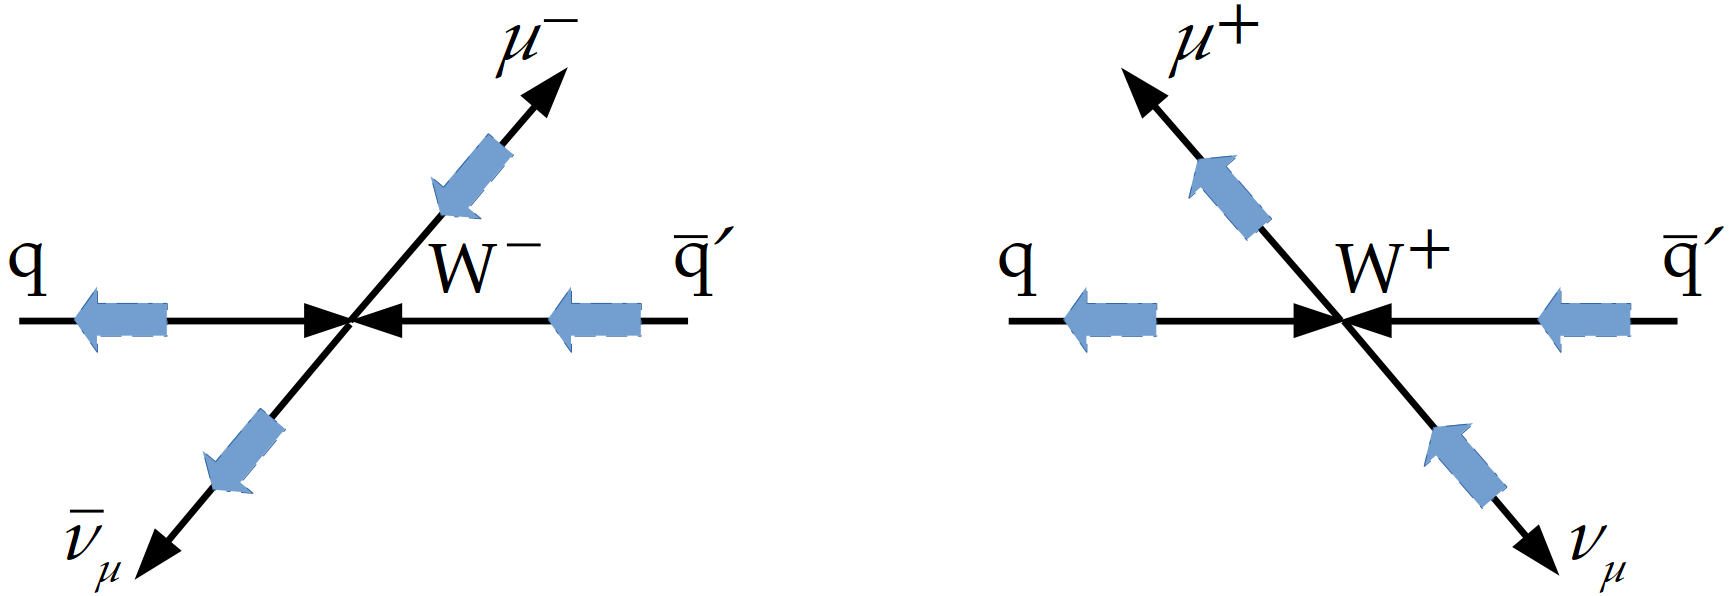
\includegraphics[width=0.8\textwidth]{Figures/WBoson/Theory/WBosonXSec.png}
 \caption{Schematic diagram of the production of \Wm (left) and \Wp (right) bosons to muonic decays. The black arrows represent the particle direction of motion whereas the blue arrows correspond to its spin. The spin of the \Wpm boson  points in the direction of the anti-quark.}
 \label{fig:WBosonXSec}
\end{figure}

At LO, the rapiditity of \Wb bosons ($y_{\Wb}$) is related to the Bjorken-x of the proton and \Pb nucleon via:

\begin{equation}
  x_{\Pp} = \frac{M_{\Wb}}{\sqrtsnn}e^{y_{\Wb}} \quad , \quad x_{\Pb} = \frac{M_{\Wb}}{\sqrtsnn}e^{-y_{\Wb}}
\end{equation}

And since the \Wb-boson rapidity is correlated to the muon $\eta$, then the pseudorapidity distribution of muons arising from \Wb-boson decays in \RunpPb collisions is sensitive to different $x$ regions of the light quark nuclear PDF that are described in the next section.


\subsection{Nuclear PDFs}\label{sec:WBoson_Introduction_nPDFs}

The parton distribution functions, introduced in \sect{sec:Physics_SI_PDF}, can not be determined from first principles due to the non-perturbative behaviour of the strong interactions. Nevertheless, their dependence on the parton momentum fraction $x$ can be derived by fitting observables (e.g. structure functions or asymmetries) to experimental data from different processes since PDFs do not depend on the initial hard scattering. The $Q^{2}$ dependence of the PDFs is determined using the DGLAP evolution equations. The most common processes used to constrain the PDFs correspond to Drell-Yan (DY), deep-inelastic scattering (DIS), vector boson and jet production, which have been measured by various experiments, including data from HERA, SLAC and LHC.

There are several proton PDF global fits currently available. In this thesis we use the NLO CT14 PDF sets published in 2016~\cite{CT14} by the collaboration of theorists and experimentalists on QCD (CTEQ). The global fits of CT14 PDFs include data of vector bosons and jets from LHC \Runpp collisions at \SI{7}{\TeV} and \SI{8}{\TeV}, charm quark DIS production from HERA, and electron charge asymmetry from Tevatron. The $x$-dependence of the CT14 PDF is parametrised at low $Q^{2}$ by~\cite{CT14}:

\begin{equation}
 xf_{a}\left(x, Q^{2}\right) = x^{c_{1}}\left(1-x\right)^{c_{2}}{P_{a}\left(x\right)}
\end{equation}

where $f_{a}$ is the PDF of a parton $a$, $c_{i}$ are parameters and $P_{a}$ is a polynomial function. In total, the CT14 proton PDFs are described by 26 parameters including: 8 parameters for the valence quarks, 5 parameters for the gluon and 13 parameters for the sea quarks~\cite{CT14}.

\fig{fig:CT14} presents the CT14 proton PDF results at $Q = \SI{2}{\GeV}$ and $Q = \SI{100}{\GeV}$. One can observe that the light valence quarks carry most of the momentum of the proton while the gluons and sea quarks are mainly distributed at low $x$. When the energy is increased, the distribution of partons gets significantly enhanced at low $x$, dominated by gluons.

\begin{figure}[!htb]
 \centering
 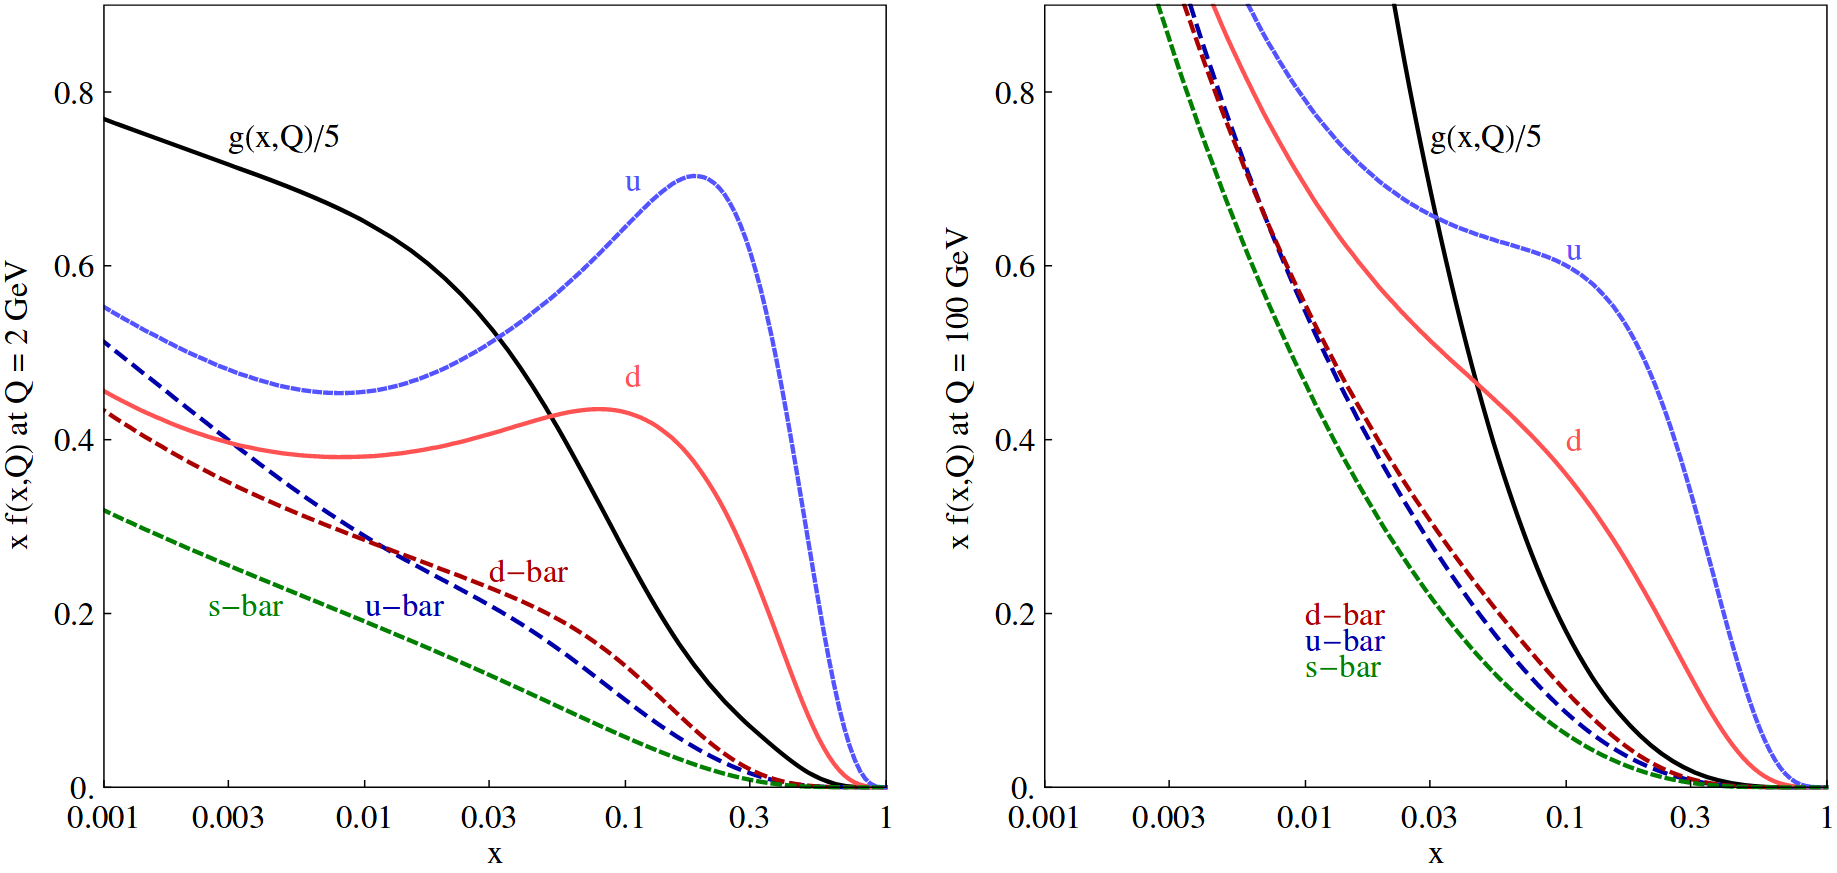
\includegraphics[width=0.9\textwidth]{Figures/WBoson/Theory/CT14NNLO.png}
 \caption{Results of the CT14 proton PDFs at NNLO derived at $Q = \SI{2}{\GeV}$ (left) and $Q = \SI{100}{\GeV}$ (right). Figures taken from Ref.~\cite{CT14}.}
 \label{fig:CT14}
\end{figure}

In heavy-ion collisions, the PDFs of the protons and neutrons bound in the nucleus are modified by the presence of the nuclear environment. The PDFs of nuclei were initially analysed in charged-lepton DIS experiments using nuclear targets by measuring the nuclear structure function per nucleon ($F^{A}_{2}$) for a heavy-ion target (A) relative to the one for deuterium ($F^{D}_{2}$)\footnote{Deuterium is approximately considered to be composed of a free proton and a free neutron.} ($R^{A}_{F_{2}} = F^{\text{A}}_{2}/F^{\text{D}}_{2}$). 

The European Muon Collaboration (EMC) measured at CERN the structure function of muon DIS from iron and deuterium targets, and published in 1983 the first observation of a depletion of the DIS cross section from iron relative to the one from deuterium in the high $x$-region $0.3 < x < 0.65$~\cite{EMCStrucFunc_1}, which was named the EMC region. Afterwards, further DIS measurements at CERN and SLAC found a suppression of the nuclear structure function compared to deuterium in the low-$x$ region $x < 0.1$ and an enhancement in the intermediate $x$-region $0.1 < x < 0.3$, which are referred as the shadowing and anti-shadowing regions~\cite{EMCStrucFunc_2}. Moreover, the measurements at SLAC using data at higher $x$ observed an increase of $R^{A}_{F_{2}}$ while approaching $x = 1$, which was expected from the motion of nucleons inside the nuclei, called Fermi motion. \fig{fig:NuclearPDFs} presents an illustration of the different regions of nuclear modifications found experimentally.

\begin{figure}[!htb]
 \centering
 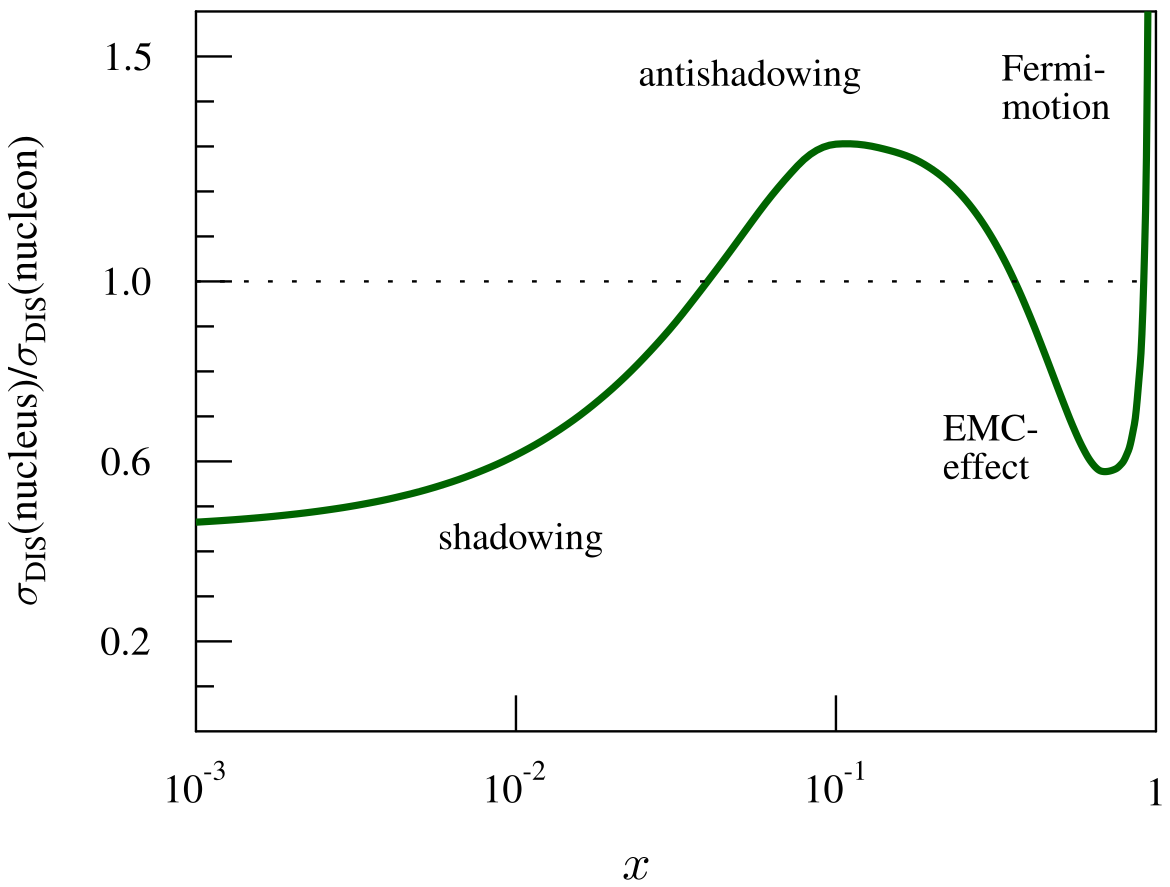
\includegraphics[width=0.45\textwidth]{Figures/WBoson/Theory/NuclearPDF.png}
 \caption{Illustration of the different nuclear PDF effects. Figure taken from Ref.~\cite{NuclearPDFIllus}.}
 \label{fig:NuclearPDFs}
\end{figure}

The different nuclear modifications can be qualitatively described as follows:

\begin{itemize}
 \item \textbf{Shadowing}: corresponds to the suppression seen in $x \lesssim 0.1$, and it arises from the multiple interactions between the scattered partons and the ones from the different nucleons. The multiple parton scatterings shifts the momentum transfer $x$ of the partons towards higher values, effectively reducing the parton densities at low $x$.
 \item \textbf{Anti-shadowing}: corresponds to an enhancement in $0.1 \lesssim x \lesssim 0.3$, and it can be understood as a consequence of the multiple parton scatterings that occur in the nucleus.
 \item \textbf{EMC effect}: corresponds to the suppression in $0.3 \lesssim x \lesssim 0.7$. Some models have been proposed to explain this phenomenon which consider modifications of the nucleon structure due to the nuclear medium and also due to short-range correlations between nucleons.
 \item \textbf{Fermi-motion effect}: corresponds to a enhancement in $x > 0.7$, and it is due to the motion of nucleons inside the nucleus.
\end{itemize}

The first global fit to describe leading-order nuclear effects was the EKS98 nPDF~\cite{EKS98}, which employed the nuclear DIS data measured at CERN and Fermilab, and the DY dimuon data from Fermilab proton-nucleus collisions. The pion data collected by RHIC was later included in subsequent global nPDF fits, such as EPS08~\cite{EPS08}, EPS09~\cite{EPS09} and DSSZ12~\cite{DSSZ12}, which provided constrains to the gluon nPDF.

The nPDFs or the nuclear modification are defined for protons bound in a nucleus. The bound neutron nPDFs are derived from the bound proton PDFs using isospin symmetry (i.e. by exchanging the up and down quark PDFs). The full nPDFs for a nucleus of $Z$ protons and $A-Z$ neutrons can be derived using the bound proton nPDFs $f^{p/A}$ and the bound neutron nPDFs $f^{n/A}$, according to:

\begin{equation}
 f^{A} = \frac{Z}{A}f^{p/Pb} + \frac{A-Z}{A}f^{n/Pb}
\end{equation}

From now on, we will focus on the latest nuclear PDF sets: the EPPS16 and nCTEQ15 nPDFs, which are used in this thesis.

\paragraph{EPPS16 nPDF.} The EPPS16 nuclear PDFs were published in 2017 by Eskola, Paakkinen, Paukkunen and Salgado~\cite{EPPS16}. By including new data and additional parameters, they replace the previous EPS09 set~\cite{EPS09}.

The EPPS16 global fits includes the same data sets as EPS09 (charged-lepton-nucleus DIS data from SLAC, DY dilepton production from EMC proton-nucleus collisions, and inclusive pion production from RHIC deuteron-nucleus collisions), as well as the CHORUS neutrino-nucleus DIS data, low-mass DY production from RHIC pion-nucleus collisions, and the results using dijet and electroweak boson production in LHC \pPb collisions at $\sqrtsnn = \SI{5.02}{\TeV}$. The addition of the new LHC, RHIC and CHORUS data into the global fit is not in tension with the previous EPS09 data sets, reassuring the validity of the universality of the nuclear PDFs. Moreover, the inclusion of the CMS measurements of the dijet pseudorapidity spectra in \pPb collisions at $\sqrtsnn = \SI{5.02}{\TeV}$~\cite{CMSDijetEta} highly constrained the gluon nPDF. On the other hand, the LHC measurements of the electroweak boson production in \pPb data did not significantly constrain the nPDF fits, mostly due to the limited statistical precision. Nevertheless, the results of the \Wb-boson production from the CMS collaboration suggested possible differences in the  modifications of the quark nPDFs. These measurements of the electroweak boson production in heavy-ion collisions at LHC will be presented in the next subsection.

The EPPS16 includes five additional parameters compared to EPS09, to account for possible flavour dependence of the quark nuclear modifications seen at LHC. The nuclear PDFs are parametrised in EPPS16 as:

\begin{equation}
  f_{i}^{p/A}\left(x,Q^{2}\right) = R_{i}^{A}\left(x,Q^{2}\right)f_{i}^{p}\left(x,Q^{2}\right)
\end{equation}

where $f_{i}^{p/A}$ represents the bound proton nPDF of parton $i$ in a nucleus A, $f_{i}^{p}$ is the free proton PDF of parton $i$ and $R_{i}^{A}$ is the corresponding nuclear correction factor. The EPPS16 nuclear modifications are derived using the NLO CT14 PDF as the free proton baseline. The parameters of $R_{i}^{A}$ are determined in three regions: the shadowing region $x\rightarrow0$, the anti-shadowing maximum point $x_{a}$ and the EMC minimum point $x_{e}$ (see \fig{fig:NuclearPDFs}). The dependence on the number of nucleons $A$ is parametrised along the three $x$ regions in the following way:

\begin{equation}
  R^{A}_{i}\left(x,Q^{2}_{0}\right) = R^{A_{\text{ref}}}_{i}\left(x,Q^{2}_{0}\right)\left(\frac{A}{A_{\text{ref}}}\right)^{\gamma_{i}\left[R_{i}^{A_{\text{ref}}}\left(x,Q^{2}_{0}\right) - 1\right]}
\end{equation}

where $Q_{0}$ is a parametrisation scale fixed at the charm pole mass (\SI{1.3}{\GeV}), $\gamma_{i}$ is a positive parameter and $A_{\text{ref}}=12$. The $Q^{2}$ dependence above $Q^{2}_{0}$ is determined by solving the DGLAP parton evolution equations. The EPPS16 nuclear modifications are parametrised in total by 20 parameters.

The EPPS16 nuclear correction factors for \Pb ions $R^{\Pb}$ extracted from the global PDF fit are shown in \fig{fig:EPPS16PDFs}. The EPPS16 results are compared against a baseline derived by performing the EPPS16 fits on the reduced dataset used in EPS09. The inclusion of these CHORUS, RHIC p-A and LHC data improves the uncertainties of the gluon $R^{A}$ at high $x$ and the strange-quark $R^{\Pb}$ at low $x$.

\begin{figure}[!htb]
 \centering
 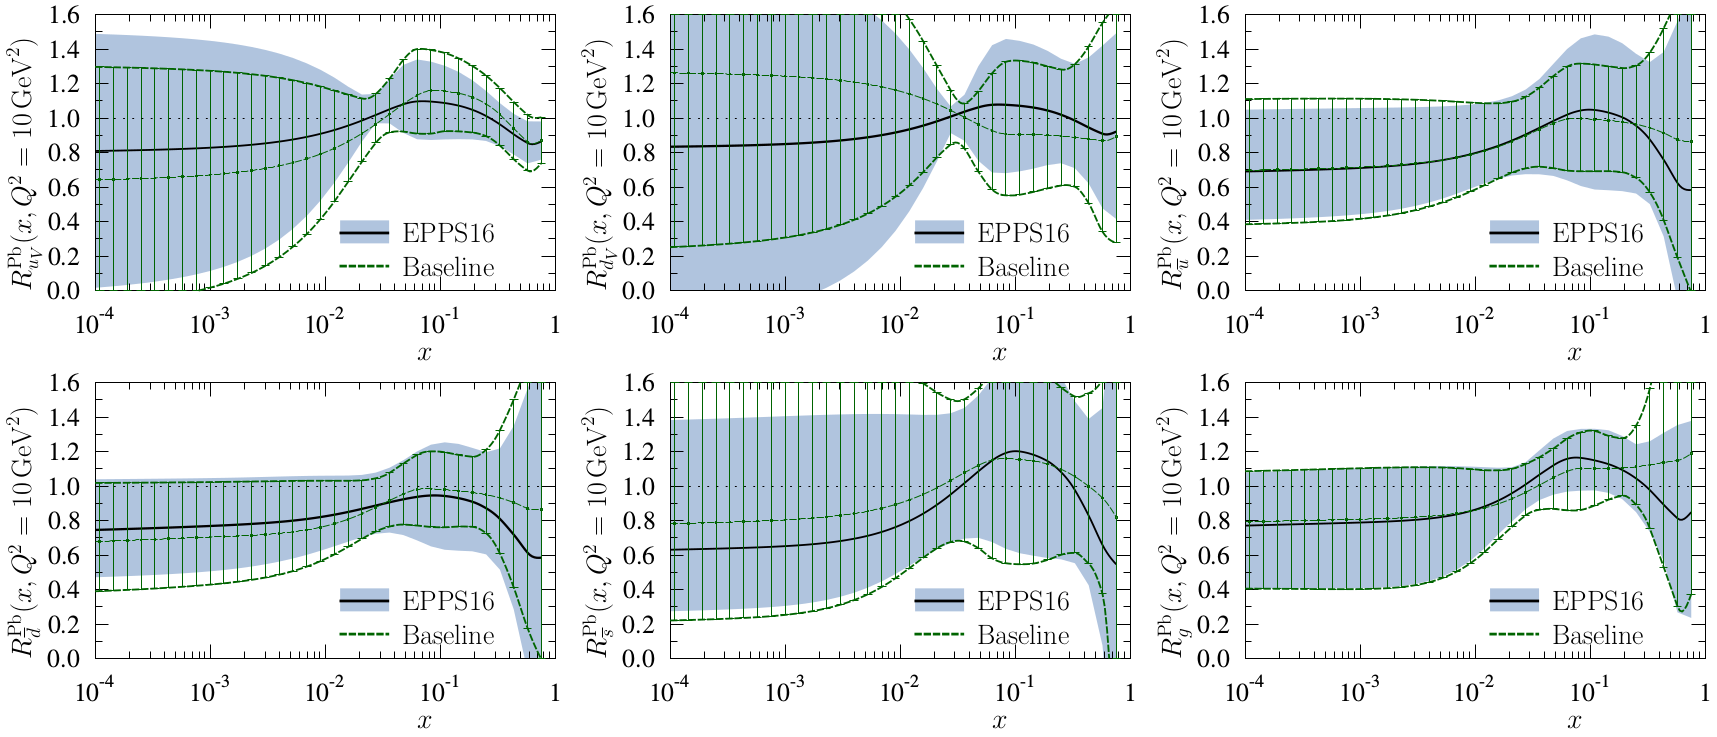
\includegraphics[width=1.0\textwidth]{Figures/WBoson/Theory/EPPS16.png}
 \caption{Results of the EPPS16 nuclear correction factor $R^{A}$ for Pb ions at $Q^{2} = \SI{10}{\square\GeV}$, corresponding to: up valence quarks (top-left), down valence quarks (top-middle), up anti-quarks (top-right), down anti-quarks (bottom-left), strange anti-quarks (bottom-middle) and gluons (bottom-right). The black curve represents the central fit while the blue bands shows the total uncertainty of the PDF fit. The results are compared against a baseline made by performing the EPPS16 fits on the same datasets used for EPS09. Figures taken from Ref.~\cite{EPPS16}.}
 \label{fig:EPPS16PDFs}
\end{figure}

\paragraph{nCTEQ15 nPDF.} The nCTEQ15 nuclear PDFs, published by Kovarik \textit{et al.} in 2016~\cite{nCTEQ15}, were derived using the CTEQ framework. The nCTEQ15 nPDF global fits make use of the charged-lepton DIS data, DY dilepton data and RHIC inclusive pion data. In contrast with EPPS16, where the nuclear modification factor $R_{i}^{p/A}$ is fitted, the nCTEQ15 global analysis parametrises the nuclear PDF $f_{i}^{p/A}$ directly (i.e. no free proton PDF is used as baseline). The nCTEQ nPDFs are parametrised as:

\begin{equation}
  \begin{alignedat}{1}
    xf_{a}^{p/A}\left(x,Q^{2}_{0}\right) &= c_{0}x^{c_{1}}\left(1-x\right)^{c_{2}}e^{c_{3}x}\left(1+e^{x_{4}}x\right)^{c_{5}} \\ 
   \frac{\cPaqd\left(x,Q^{2}_{0}\right)}{\cPaqu\left(x,Q^{2}_{0}\right)} &= c_{0}x^{c_{1}}\left(1-x\right)^{c_{2}} + \left(1+c_{3}x\right)\left(1-x\right)^{c_{4}}
  \end{alignedat}
\end{equation}

where $f_{a}^{p/A}$ is the bound proton nPDF of a parton $a$ in a nucleus A, {\cPaqd} and {\cPaqu} are the down and up anti-quark nPDFs, respectively, $c_{i}$ are parameters, and the parametrisation scale $Q_{0}$ is fixed at $\SI{1.3}{\GeV}$. The strange quark and anti-quark nPDFs are assumed to be the same. The $A$-dependence of the nPDFs is parametrised in nCTEQ15 using the coefficients $c_{i}$, according to:

\begin{equation}
 c_{i}\left(A\right) = c_{i,0} + c_{i,1}\left(1-A^{-c_{i,2}}\right)
\end{equation}

The nCTEQ15 fits are performed using 16 free parameters. In addition, the nCTEQ15 treats the up and down  valence quark PDFs independently but it assumes no flavour dependence for nuclear modifications of the up and down anti-quarks.

\fig{fig:nCTEQ15} shows the nCTEQ15 results of the full nuclear lead PDFs $f^{\Pb}$ at $Q = \SI{10}{\GeV}$ compared to the results from the EPS09 and HKN07~\cite{HKN07} nPDFs. One can see that at $x \gtrsim 0.05$ the up and down valence quark nPDFs dominates while at $x < 0.01$ the sea quarks and the gluons nPDFs become dominant.

\begin{figure}[!htb]
 \centering
 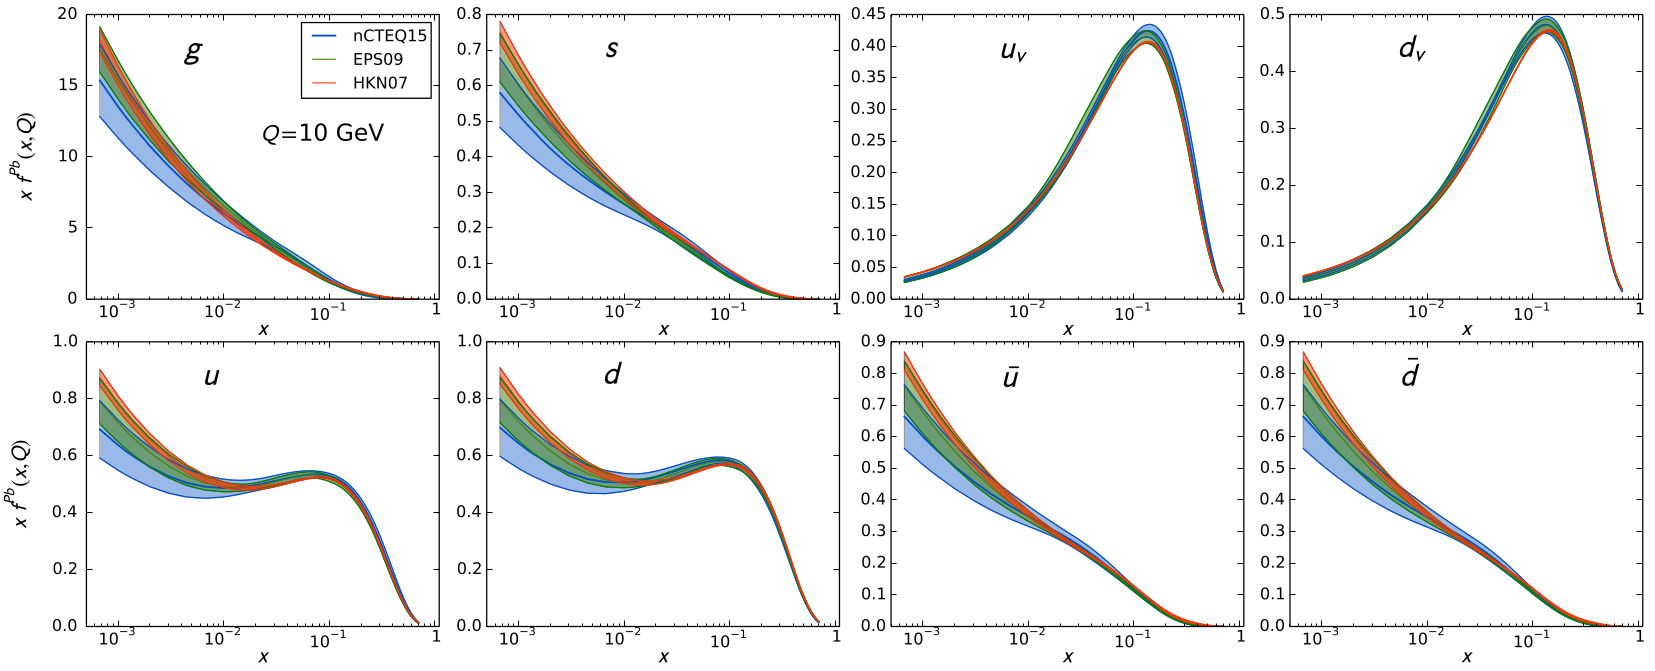
\includegraphics[width=1.0\textwidth]{Figures/WBoson/Theory/nCTEQ15.png}
 \caption{Results of the nCTEQ15 full nuclear PDFs for \Pb ions $f^{\Pb}$ at $Q = \SI{10}{\GeV}$ (blue curve with band), compared to the corresponding ones from EPS09~\cite{EPS09} (green curve with band) and HKN07~\cite{HKN07} (orange curve with band). The plots, in order from top-left to bottom-right, correspond to: gluons, strange quarks, up valence quarks, down valence quarks, up quarks, down quarks, up anti-quarks and down anti-quarks. Figures taken from Ref.~\cite{nCTEQ15}.}
 \label{fig:nCTEQ15}
\end{figure}

A comparison between the results of the nCTEQ15 and EPPS16 nuclear modifications at $Q = \SI{100}{\GeV}$ is shown in \fig{fig:EPPS16vsnCTEQ15}. The nCTEQ15 central set expects more shadowing at low $x$ than EPPS16 for the down valence quarks, while the opposite trend is observed for up valence quarks. Moreover, the uncertainties of the EPPS16 calculations are much larger than the nCTEQ15 ones because the EPPS16 uses more parameters to fit the nuclear modifications.

\begin{figure}[!htb]
 \centering
 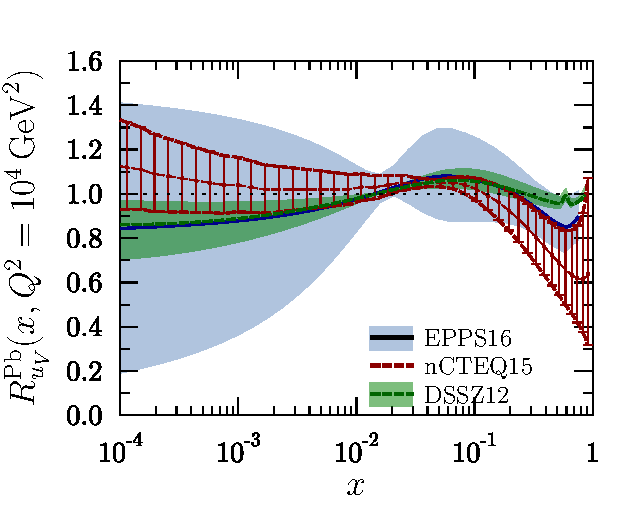
\includegraphics[width=0.32\textwidth]{Figures/WBoson/Theory/EPPS16/Pb_uv_highQ_comp.pdf}
 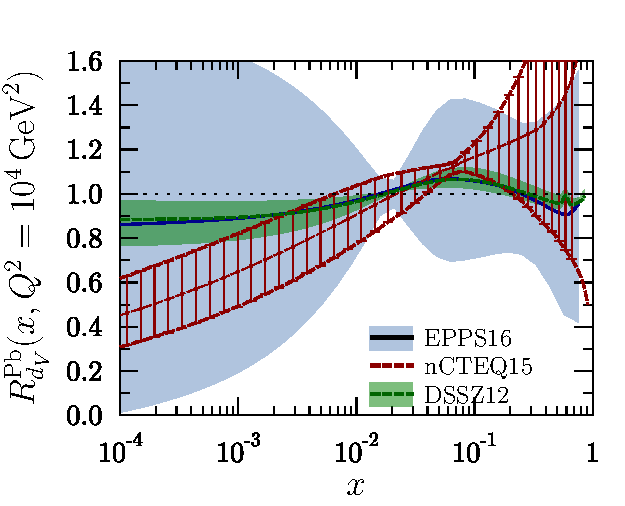
\includegraphics[width=0.32\textwidth]{Figures/WBoson/Theory/EPPS16/Pb_dv_highQ_comp.pdf}
 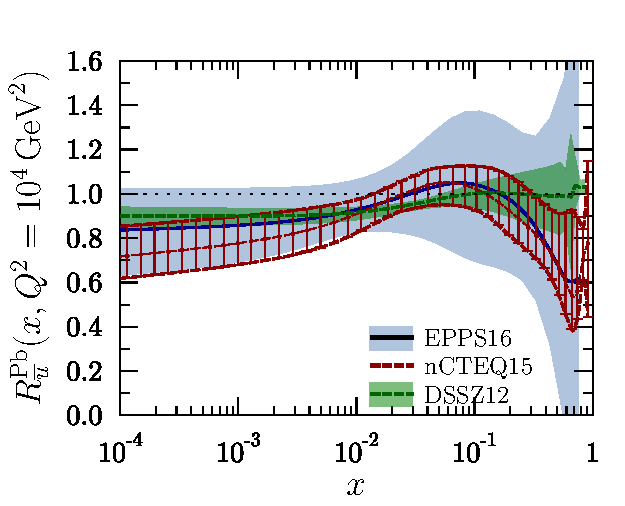
\includegraphics[width=0.32\textwidth]{Figures/WBoson/Theory/EPPS16/Pb_us_highQ_comp.pdf}
 \\
 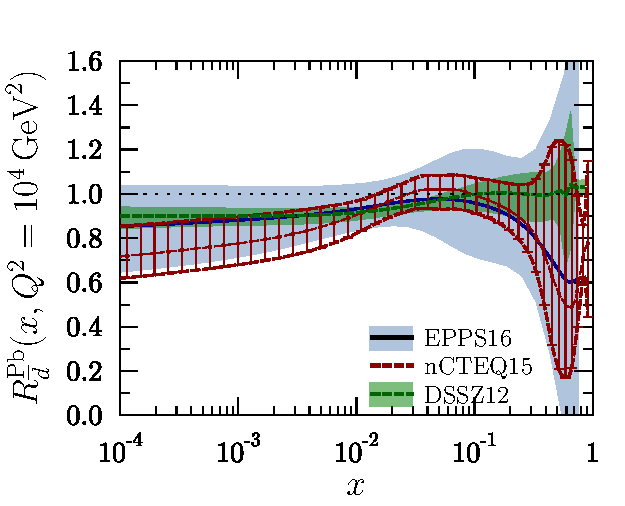
\includegraphics[width=0.32\textwidth]{Figures/WBoson/Theory/EPPS16/Pb_ds_highQ_comp.pdf}
 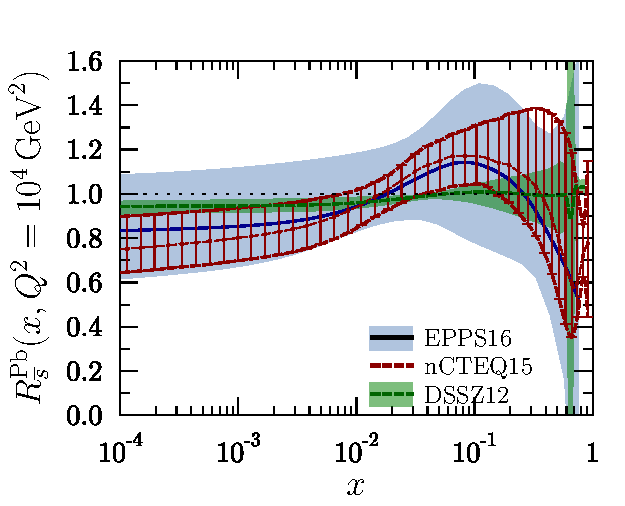
\includegraphics[width=0.32\textwidth]{Figures/WBoson/Theory/EPPS16/Pb_ss_highQ_comp.pdf}
 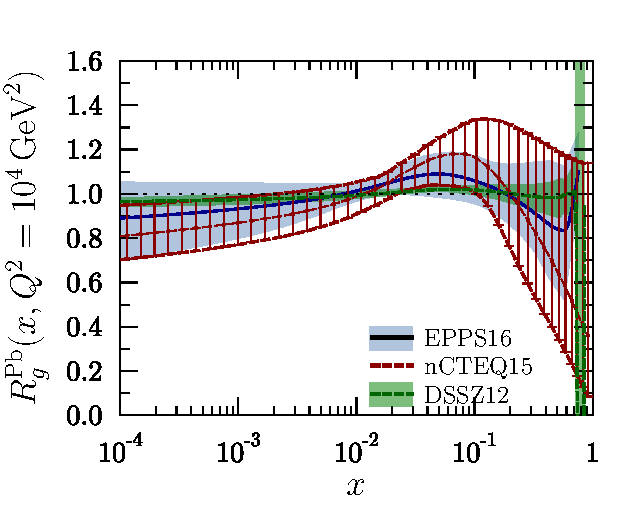
\includegraphics[width=0.32\textwidth]{Figures/WBoson/Theory/EPPS16/Pb_g_highQ_comp.pdf}
 \caption{Comparison between the EPPS16 (blue curve with band), nCTEQ15 (red curves with hatching) and DSSZ12 (green curve with band) nuclear modifications performed at $Q^{2} = 10^{4}~\si{\square\GeV}$, corresponding to: up valence quarks (top-left), down valence quarks (top-middle), up anti-quarks (top-right), down anti-quarks (bottom-left), strange anti-quarks (bottom-middle) and gluons (bottom-right). Figures provided by the EPPS16 authors.}
 \label{fig:EPPS16vsnCTEQ15}
\end{figure}

The main characteristics of the EPS09, EPPS16 and nCTEQ15 nuclear PDFs are summarized in \tab{tab:nPDFInfo}.

\begin{table}[htbp]
  \centering
  \begin{tabular}{ c | c c c }
   nPDF & EPS09 & EPPS16 & nCTEQ15 \\ \hline
   Order & NLO & NLO & NLO \\
   Fit & nucler modification & nuclear modification & nuclear PDF \\
   Baseline PDF & CTEQ6 & CT14 & \\
   Free parameters & 15 & 20 & 17 \\
   Data points & 929 & 1811 & 708 \\
   EMC DY dileptons in p-A & Yes & Yes & Yes \\
   RHIC pions in d-A & Yes & Yes & Yes \\
   SLAC $l^{\pm}$-A DIS & Yes & Yes & Yes \\
   CHORUS $\nu$-A DIS & No & Yes & No \\
   RHIC DY in $\pi$-A & No & Yes & No \\
   LHC dijets in \pPb & No & Yes & No \\
   LHC weak bosons in \pPb & No & Yes & No
  \end{tabular}
  \caption{Summary of the information of EPS09, EPPS16 and nCTEQ15 nuclear PDFs.}
  \label{tab:nPDFInfo}
\end{table}


\subsection{Experimental results at LHC}\label{sec:WBoson_Introduction_Results}


Measurements of the weak boson production in heavy-ion collisions have been performed by the LHC experiments. The latest results have been derived from \RunpPb collisions at $\sqrtsnn = \SI{5.02}{\TeV}$ and \RunPbPb collisions at $\sqrtsnn = \SI{2.76}{\TeV}$ and $\sqrtsnn = \SI{5.02}{\TeV}$. This subsection gives a brief summary on some of the results.

\paragraph{\RunPbPb results.}  The CMS~\cite{CMS_W_PbPb_2p76TeV,CMS_Z_PbPb_2p76TeV} and ATLAS~\cite{ATLAS_W_PbPb_2p76TeV,ATLAS_Z_PbPb_2p76TeV} collaborations measured the \Wb- and \Z-boson production in \RunPbPb collisions at $\sqrtsnn = \SI{2.76}{\TeV}$ in the lepton decay channel. The ATLAS and CMS measurements were performed in the mid-rapidity region ($\abs{y} < 2.5$). The results are in good agreement with NLO pQCD calculations with and without nuclear PDF corrections. Moreover, the centrality dependence of the weak boson yields is observed to scale with \ncoll, within uncertainties. In the case of \Wb boson, the lepton charge asymmetry of \Wpm, defined as $(N^{+}_{\ell} - N^{-}_{\ell})/(N^{+}_{\ell} + N^{-}_{\ell})$, is found to be different from the results in \Runpp collisions, but this is understood to be simply associated to the different number of protons and neutrons in the \Pb nuclei, the isospin effect. The statistical precision of the results is not enough to provide significant constrains on the global fits to the PDFs.

Results from the ALICE collaboration extend the measurements on the production of \Z bosons in \RunPbPb collisions at $\sqrtsnn = \SI{5.20}{\TeV}$~\cite{ALICE_Z_PbPb_5p02TeV} in the low Bjorken-$x$ forward rapidity region ($2.5 < y < 4.0$), where more shadowing is expected. The measurements deviate significantly ($\sim$3 standard deviations) from calculations assuming only isospin effects and agree with calculations including nuclear PDF corrections.


\paragraph{\RunpPb results.} The ATLAS collaboration has measured the \Z-boson production in \RunpPb collisions at $\sqrtsnn = \SI{5.02}{\TeV}$~\cite{ATLAS_Z_pPb_5p02TeV}. The \Z-boson cross section  as a function of the \Z-boson rapidity determined in the centre-of-mass frame, is displayed in \fig{fig:ATLAS_Z_pPb_5p02TeV}. The results are better described by the PDF model calculations including nuclear modifications, although the free-proton PDF calculations are not excluded within the precision of the measurement.

\begin{figure}[!htb]
 \centering
 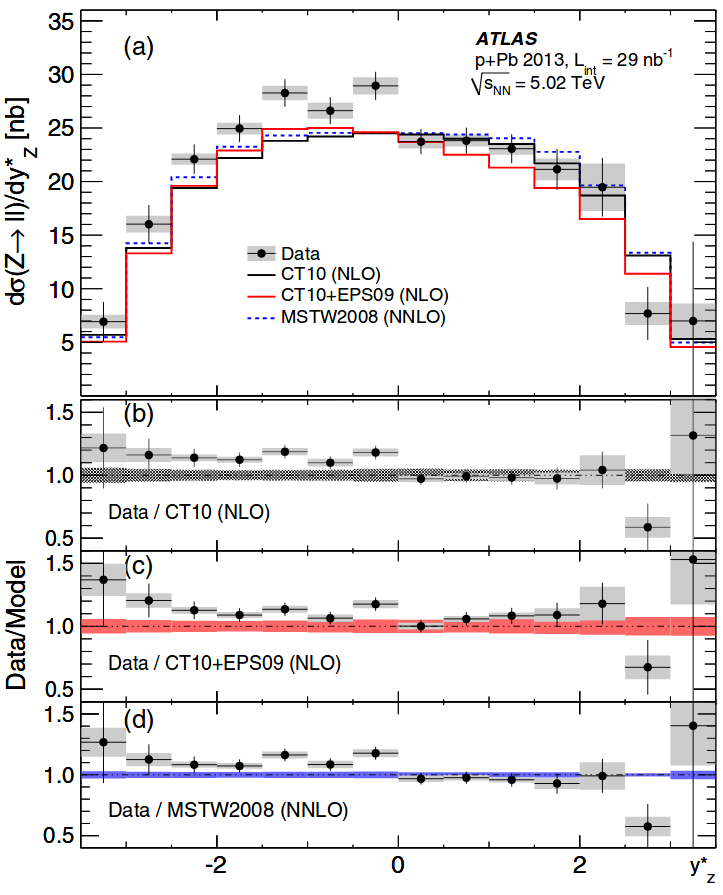
\includegraphics[width=0.45\textwidth]{Figures/WBoson/Theory/ATLAS_Z_XSec.png}
 \caption{Distribution of the production cross section for $\ZToMuMu$ measured in \RunpPb collisions at $\sqrtsnn = \SI{5.02}{\TeV}$ as a function of the \Z-boson rapidity in the centre-of-mass frame. Figure taken from Ref.~\cite{ATLAS_Z_pPb_5p02TeV}.}
 \label{fig:ATLAS_Z_pPb_5p02TeV}
\end{figure}

The CMS and ALICE collaborations have published results on the production of \Wb bosons in \RunpPb collisions at $\sqrtsnn = \SI{5.02}{\TeV}$~\cite{HIN-13-007,ALICE_W_pPb_5p02TeV}. The measurements of the \Wb-boson production cross section performed by the ALICE collaboration~\cite{ALICE_W_pPb_5p02TeV}, as a function of the lepton rapidity in the centre-of-mass frame, are shown in \fig{fig:ALICE_W_pPb_5p02TeV}. The ALICE results are compared to NLO calculations using the CT10 proton PDF and NNLO calculations using the FEWZ generator and the MSTW200 proton PDF, with and without EPS09 nuclear PDF corrections. The cross section results are found to be in good agreement with the NLO model calculations while NNLO calculations without nuclear PDF modifications slightly overestimate the measurement at forward lepton rapidity ($2.03 < \abs{y_{\text{cms}}} < 3.53$).

\begin{figure}[!htb]
 \centering
 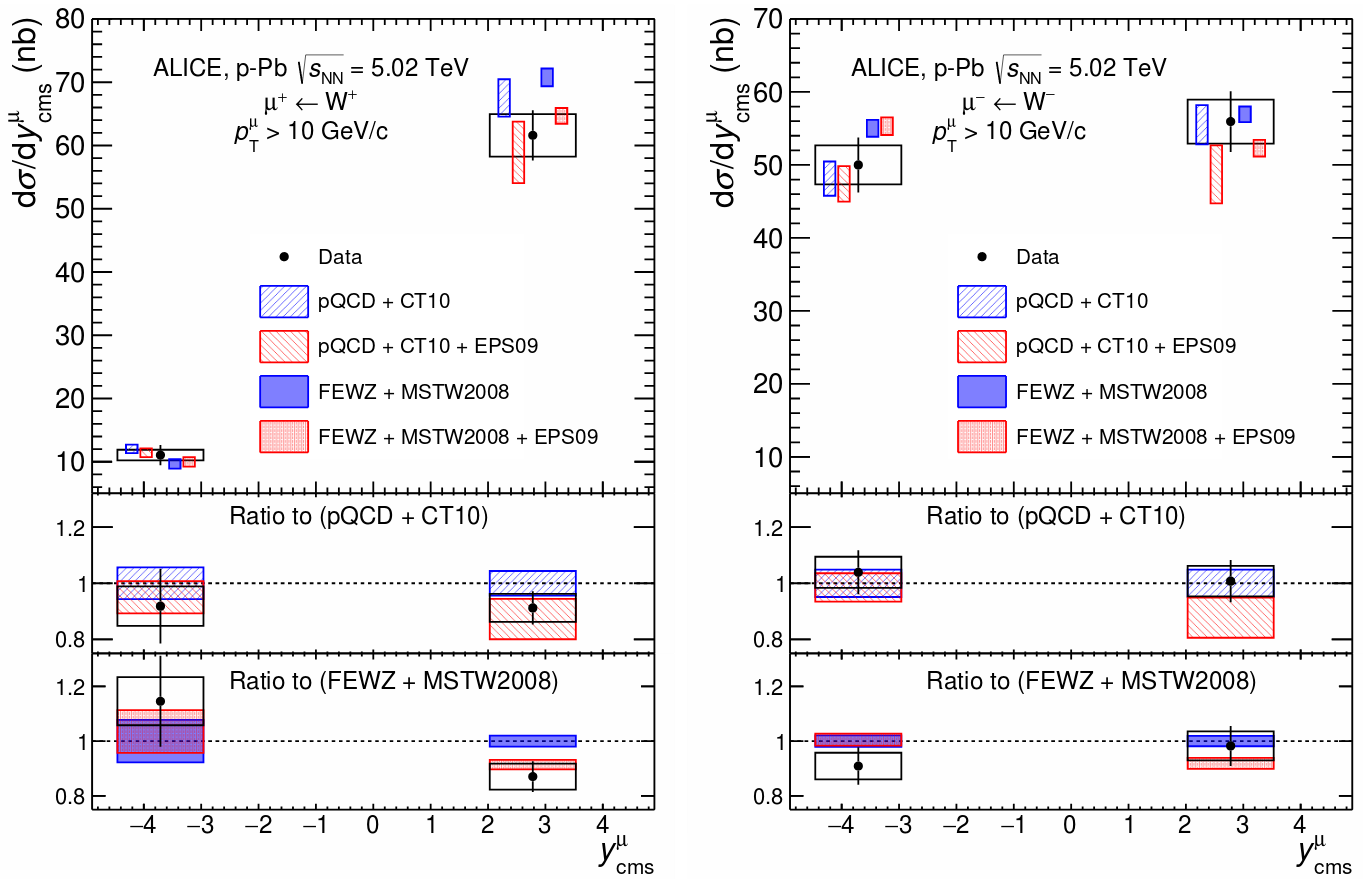
\includegraphics[width=0.66\textwidth]{Figures/WBoson/Theory/Cross_Section_ALICE.png}
 \caption{Distribution of the production cross section for $\WToMuNuMi$ (left) and $\WToMuNuPl$ (right) measured in \RunpPb collisions at $\sqrtsnn = \SI{5.02}{\TeV}$ as a function of the muon rapidity in the centre-of-mass frame. Figures taken from Ref.~\cite{ALICE_W_pPb_5p02TeV}.}
 \label{fig:ALICE_W_pPb_5p02TeV}
\end{figure}

Finally, the \Wb-boson measurements of CMS~\cite{HIN-13-007} are performed in the muon and electron decay channels as a function of the lepton pseudorapidity in the laboratory frame~\cite{HIN-13-007}. \fig{fig:CMS_W_pPb_5p02TeV} shows the measured cross sections for $\Wm\rightarrow\ell^{-}\overline{\nu}_{\ell}$ (left) and $\Wp\rightarrow\ell^{+}{\nu}_{\ell}$ (middle), and the lepton charge asymmetry (right), compared to the NLO pQCD calculations using the CT10 proton PDF with and without EPS09 nuclear corrections. Both theoretical calculations are found to be in good agreement with the measured cross sections within uncertainties, except in the backward region ($\etaLAB < -1.0$) for \Wm bosons, where a small excess is seen in the results. The small deviation is also reflected in the measured lepton charge asymmetry, where the model calculations overestimate the data in the region $-2.0 < \etaLAB < -1.0$. It was suggested at the time that the small disagreement between the PDF calculations and the data could be due to different flavour dependence between the up and down quark PDFs~\cite{HIN-13-007}.

\begin{figure}[!htb]
 \centering
 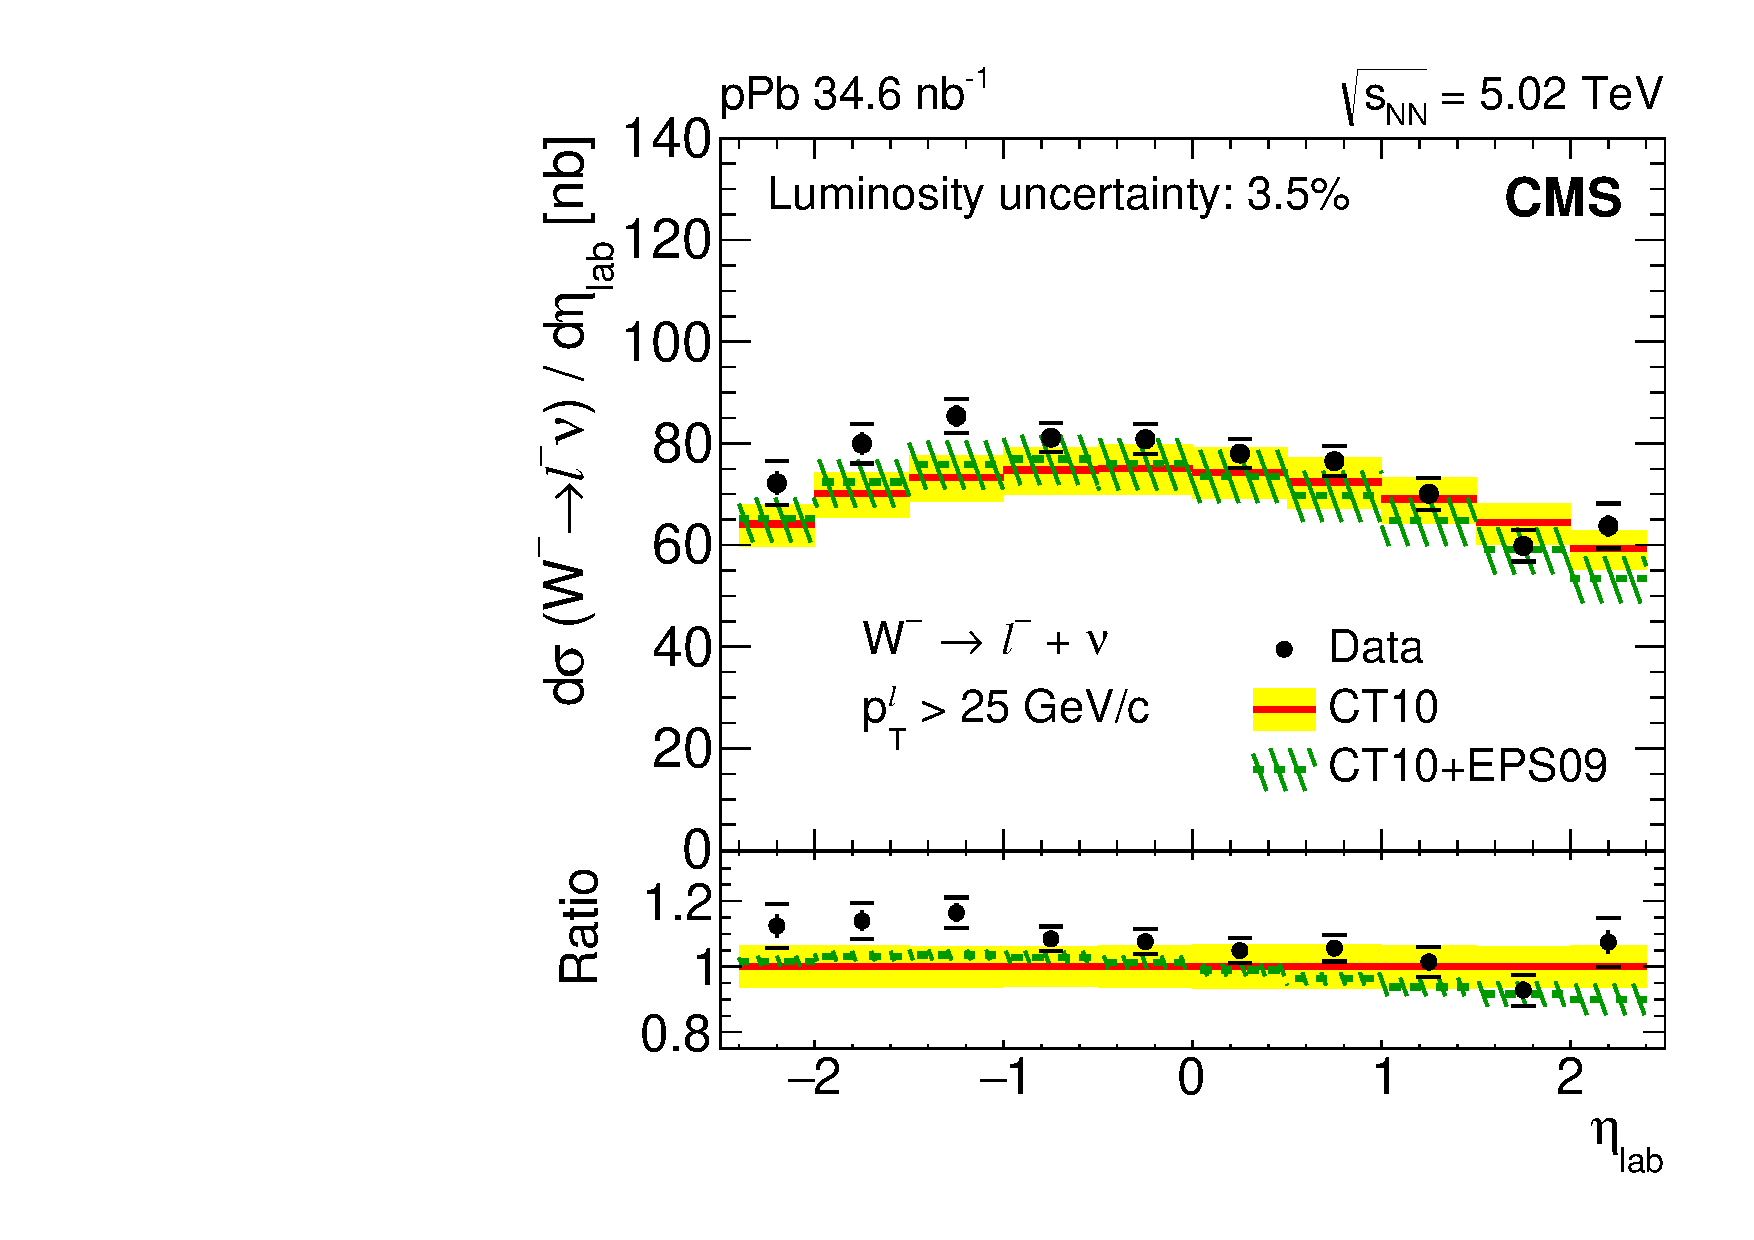
\includegraphics[width=0.32\textwidth]{Figures/WBoson/Theory/CMS_W_5p02TeV_XSec_Wm.pdf}
 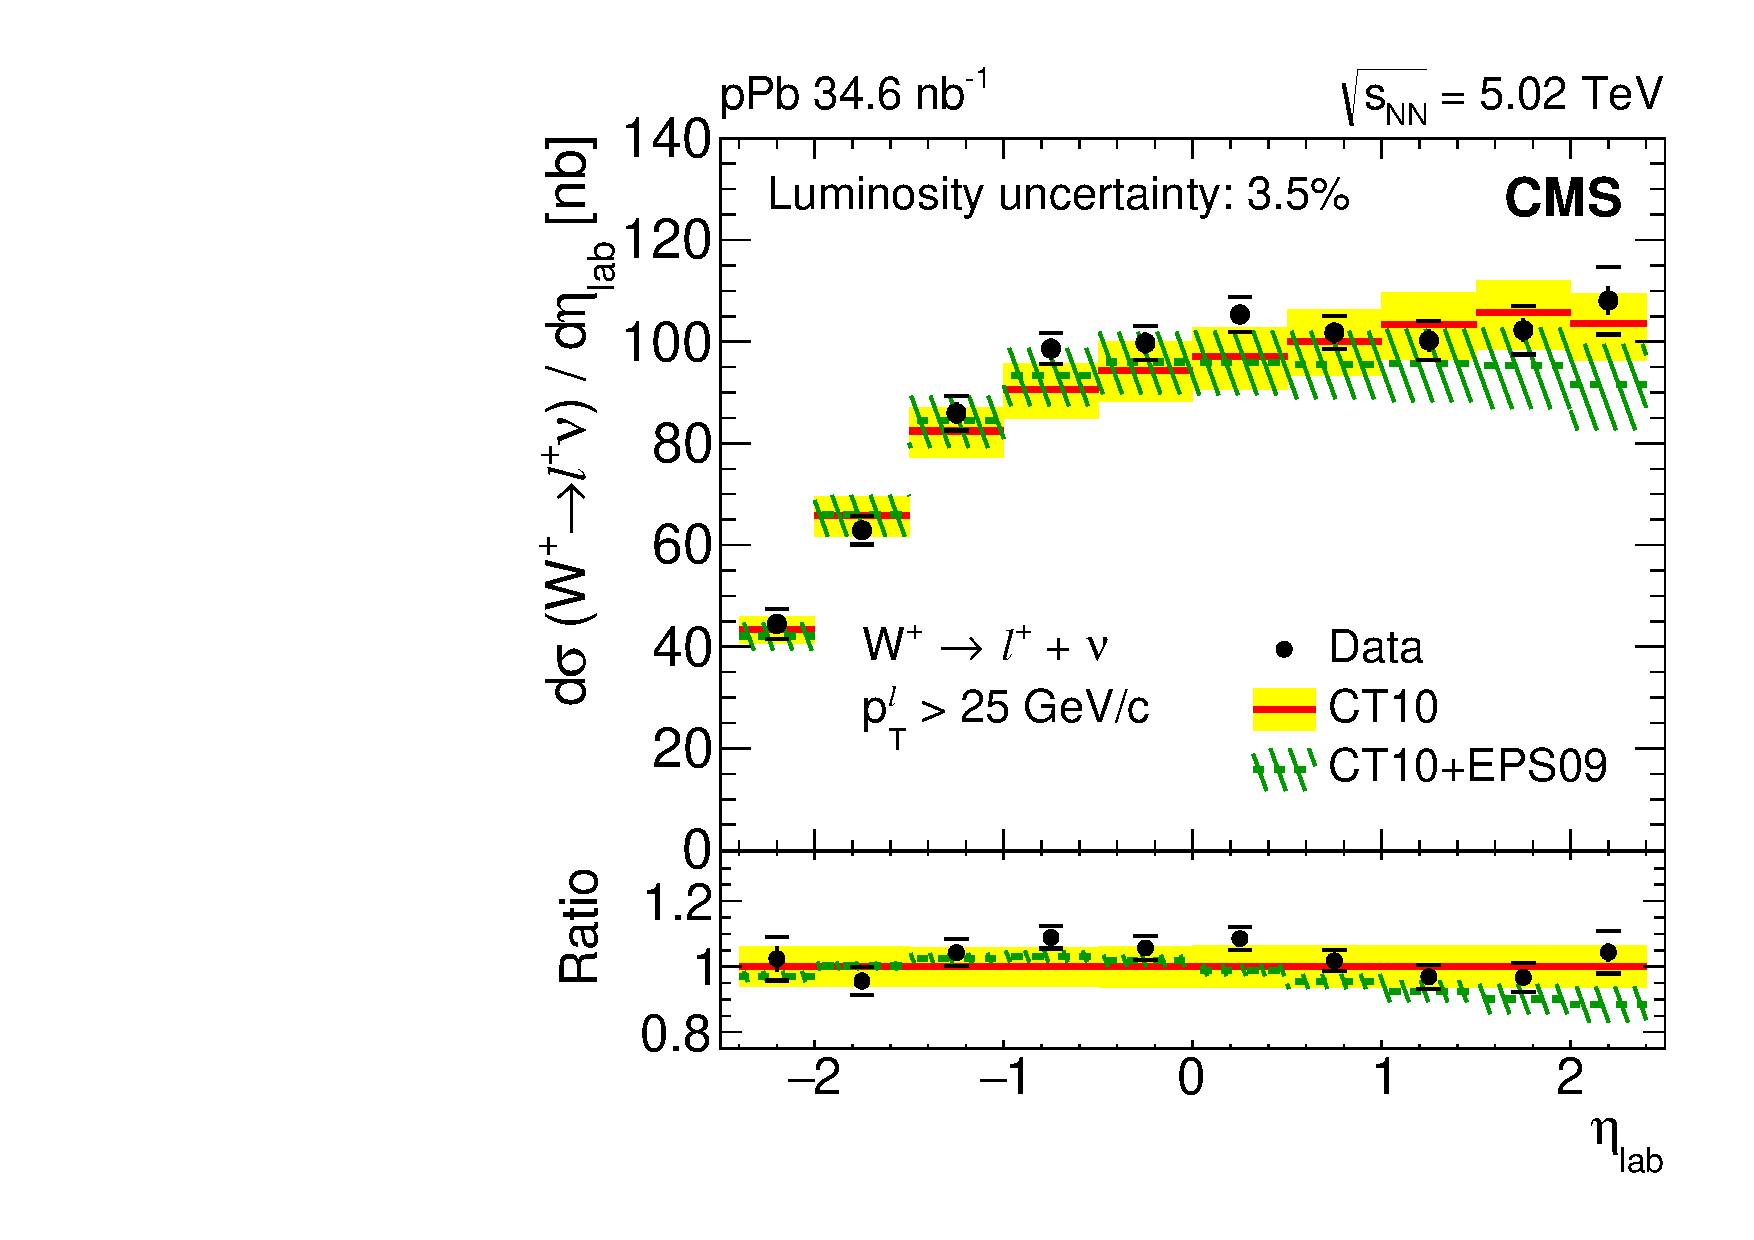
\includegraphics[width=0.32\textwidth]{Figures/WBoson/Theory/CMS_W_5p02TeV_XSec_Wp.pdf}
 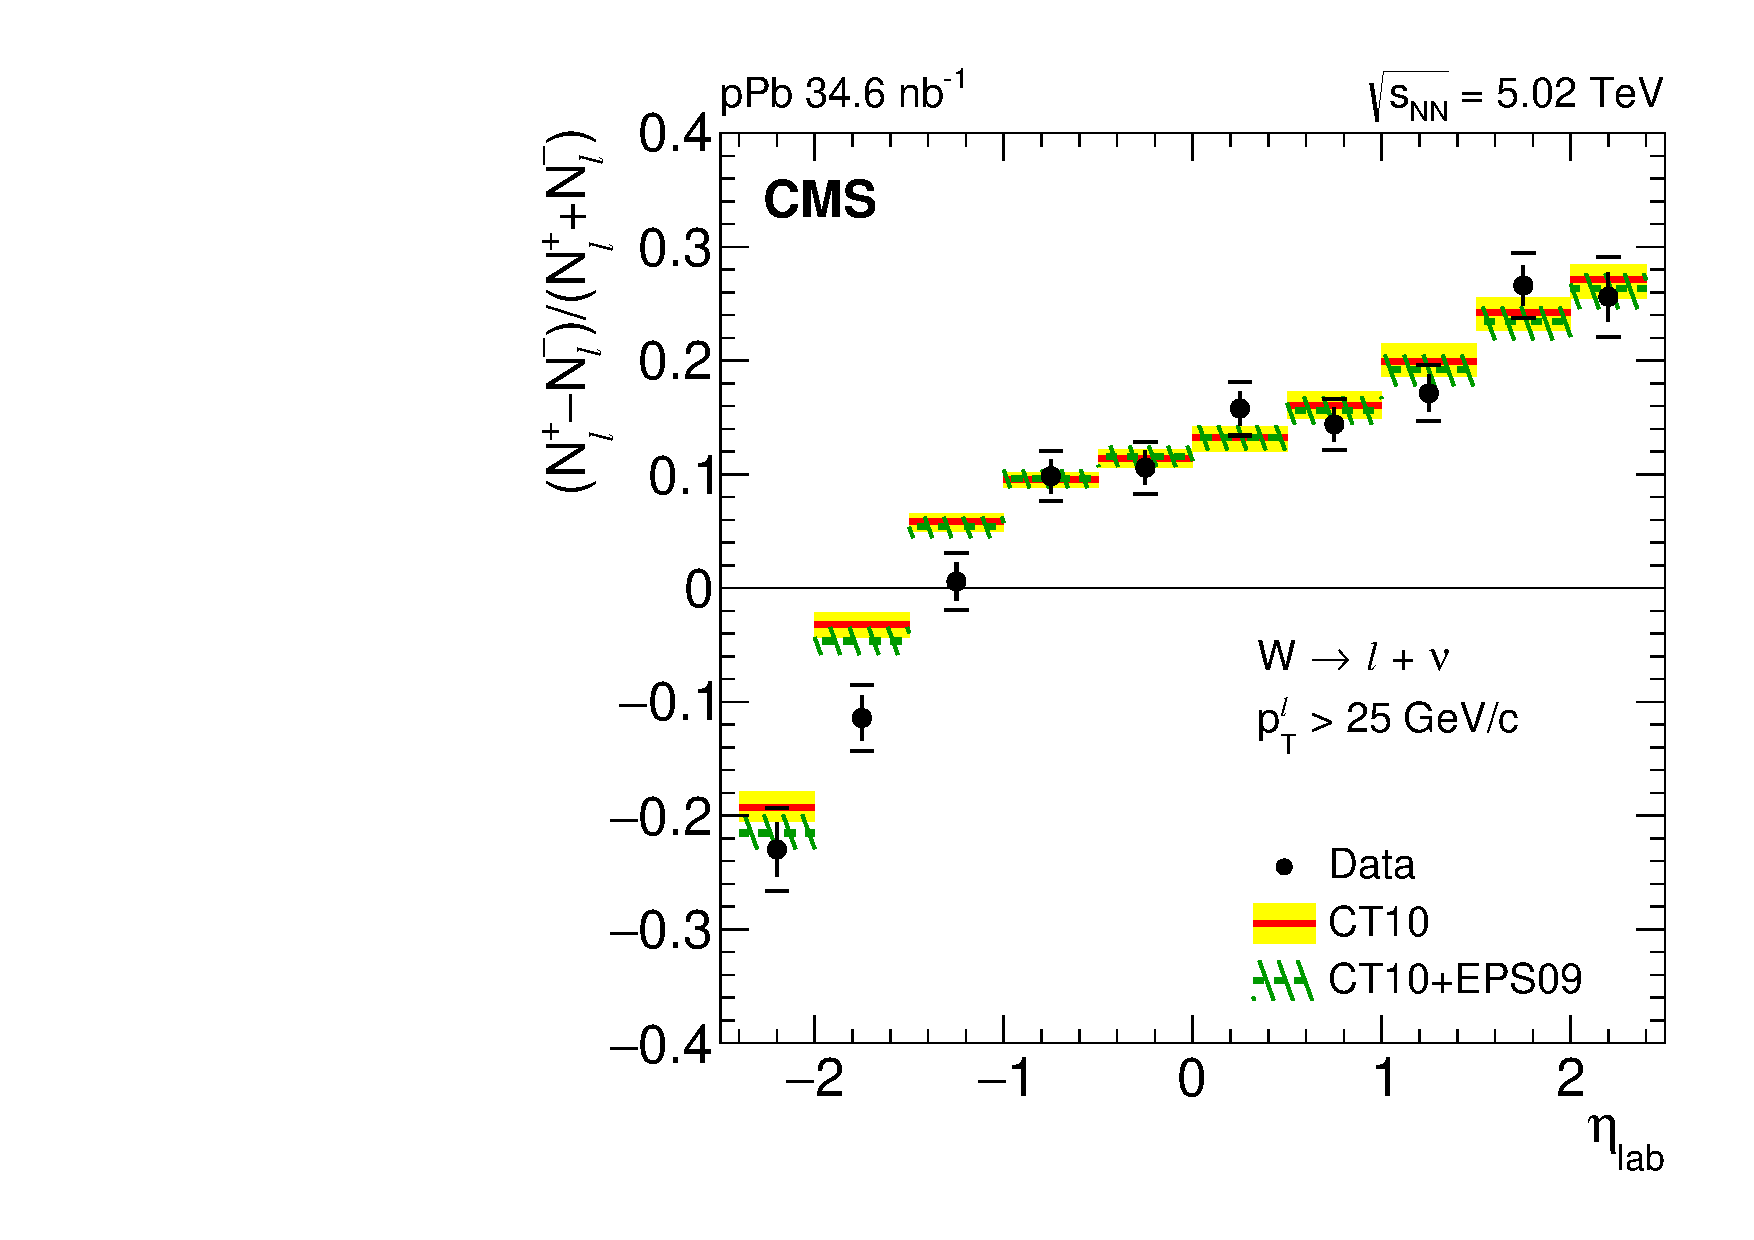
\includegraphics[width=0.32\textwidth]{Figures/WBoson/Theory/CMS_W_5p02TeV_ChgAsym.pdf}
 \caption{Distribution of the production cross section for $\Wm\rightarrow\ell^{-}\overline{\nu}_{\ell}$ (left) and $\Wp\rightarrow\ell^{+}{\nu}_{\ell}$ (middle), and the lepton charge asymmetry (right) measured in \RunpPb collisions at $\sqrtsnn = \SI{5.02}{\TeV}$ as a function of the lepton pseudorapidity in the laboratory frame. The CT10 PDF calculations with EPS09 (green line) and without (red line) nuclear PDF corrections are included. The bottom panels present the ratio of the CT10+EPS09 (green line) and data (black points) normalised to the CT10 baseline. Figures taken from Ref.~\cite{HIN-13-007}.}
 \label{fig:CMS_W_pPb_5p02TeV}
\end{figure}

% END OF SECTION
